%% New Glenn static-fire explosion seismo-acoustic paper -- Seismica submission format (FIRST DRAFT)
%% Compile from this directory:  ./compile2.sh NewGlenn_explosion_paper.tex
%% Needs seismica.cls, abbrvnat_seismica_upcasetitle.bst and banner.png here.
%%
%% Numbers in this draft come from the notebooks in this folder (run 2026-11-23):
%%   21 station map, 22 data overview, 24 origin time, 26 seismic arrivals, 28 coupling,
%%   30 spectral ratios, 32 Chaparral sensitivity, 34 amplitude vs distance,
%%   36 velocity model (verticals), 38 horizontals and joint model.

\documentclass[]{seismica}

\usepackage{amssymb}
\usepackage{booktabs}
\usepackage{array}
\usepackage{subcaption}

\newcommand{\todo}[1]{\textcolor{red}{\textbf{[TODO: #1]}}}
\newcommand{\placeholder}[1]{\textcolor{orange}{\textbf{[#1]}}}
\newcommand{\suppfig}[1]{Figure~S#1}
\newcommand{\supptab}[1]{Table~S#1}

\graphicspath{{figures/}}

%% Key numbers, generated by 42_paper_numbers.ipynb from the notebooks' outputs
% Generated by 42_paper_numbers.ipynb from the notebooks' outputs; do not edit by hand.
\newcommand{\NGorigin}{01:00:02.4}
\newcommand{\NGoriginPrecise}{01:00:02.37}
\newcommand{\NGoriginSpread}{0.27}
\newcommand{\NGoriginRange}{01:00:02.2--03.2}
\newcommand{\NGoriginFree}{01:00:01.2}
\newcommand{\NGspeedFree}{339}
\newcommand{\NGtemp}{26.4}
\newcommand{\NGrh}{87}
\newcommand{\NGpressure}{1014}
\newcommand{\NGwind}{2.2}
\newcommand{\NGwindFrom}{298}
\newcommand{\NGczero}{348.7}
\newcommand{\NGceff}{346.7--347.3}
\newcommand{\NGheadwind}{1.5--2.0}
\newcommand{\NGpBtwenty}{407}
\newcommand{\NGpFar}{264--342}
\newcommand{\NGtpos}{0.36--0.44}
\newcommand{\NGipos}{28--61}
\newcommand{\NGiposr}{580--1050}
\newcommand{\NGnegRatio}{3--7}
\newcommand{\NGnPeak}{0.58 \pm 0.15}
\newcommand{\NGnLow}{1.23 \pm 0.09}
\newcommand{\NGnImp}{1.2 \pm 0.4}
\newcommand{\NGnPeakCorr}{1.15}
\newcommand{\NGdecBfourteen}{26--28}
\newcommand{\NGdecOther}{1--4}
\newcommand{\NGdecMax}{28}
\newcommand{\NGyieldP}{145}
\newcommand{\NGyieldPrange}{94--246}
\newcommand{\NGyieldT}{376}
\newcommand{\NGyieldTrange}{307--573}
\newcommand{\NGzRange}{200--320}
\newcommand{\NGyieldVsSilber}{11}
\newcommand{\NGcompBfourteen}{-75}
\newcommand{\NGcompBfourteenRange}{$-60$ to $-78$}
\newcommand{\NGcompBtwentynine}{-68}
\newcommand{\NGcompBzerofive}{-17}
\newcommand{\NGcompRange}{17--78}
\newcommand{\NGkRms}{1.8--5.3}
\newcommand{\NGkPeak}{1.1--3.9}
\newcommand{\NGcompAtwoBzerofive}{-15.9}
\newcommand{\NGcompAtwoBtwentynine}{-65.9}
\newcommand{\NGcompAgree}{6}
\newcommand{\NGfzero}{4.5--5.5}
\newcommand{\NGfirstArrival}{5.5--9.2}
\newcommand{\NGvFirst}{2.1--3.8}
\newcommand{\NGlead}{47--55}
\newcommand{\NGvsTop}{330--560}
\newcommand{\NGtopThick}{30--50}
\newcommand{\NGhalfDepth}{305--385}
\newcommand{\NGvsHalf}{1610}
\newcommand{\NGchapEarly}{0.36--0.42}
\newcommand{\NGchapLate}{0.39--0.46}
\newcommand{\NGchapExplosion}{0.022}
\newcommand{\NGchapWindows}{354}
\newcommand{\NGchapLaunches}{41}


\title{Seismo-acoustic recordings of the May~2026 New~Glenn static-fire explosion at Cape~Canaveral: blast wave, air-to-ground coupling and seismic waves ahead of the airwave}
\shorttitle{The New Glenn static-fire explosion}

\author[1]{Glenn Thompson\thanks{Corresponding author: \texttt{thompsong@usf.edu}; ORCID: 0000-0002-9173-0097}}
\author[2]{Paul Bremner}
\author[2]{Han Byul Woo}
\author[3]{Sue Bilek}
\affil[1]{School of Geosciences, University of South Florida, Tampa, Florida, USA}
\affil[2]{NASA Marshall Space Flight Center, Huntsville, Alabama, USA}
\affil[3]{New Mexico Institute of Mining and Technology, Socorro, New Mexico, USA}

\credit{Conceptualization}{Glenn Thompson}
\credit{Methodology}{Glenn Thompson}
\credit{Software}{Glenn Thompson}
\credit{Formal Analysis}{Glenn Thompson}
\credit{Investigation}{Glenn Thompson}
\credit{Resources}{Glenn Thompson}
\credit{Data Curation}{Glenn Thompson}
\credit{Visualization}{Glenn Thompson}
\credit{Project Administration}{Glenn Thompson}
\credit{Writing - Original draft}{Glenn Thompson}
\credit{Writing - Review \& Editing}{Glenn Thompson, Paul Bremner, Han Byul Woo, Sue Bilek}

\begin{document}

\makeseistitle{
  \begin{summary}{Abstract}
  %% DRAFT
  A Blue Origin New~Glenn rocket exploded on Launch Complex~36 at Cape
  Canaveral during a static-fire test at about 01:00~UTC on 29~May~2026.
  \NGnStationsCap{} broadband seismo-acoustic stations of a network installed for
  the Artemis~II launch were still recording \NGdistRange~km away; \NGnWorking{} had
  working sensors. Using the airwave arrival times and the speed of sound
  predicted from surface weather, we place the origin at
  \NGorigin~UTC~$\pm$~1~s; allowing for the supersonic blast front near the
  pad moves it to \NGoriginCorrRange, \NGflashGapRange~s before the main flash seen on video.
  Peak overpressures were \NGpBtwenty~Pa at \NGdistBtwenty~km and
  \NGpFar~Pa at \NGfarRange~km. Below 4~Hz the airwave decays close to
  spherical spreading, but above 4~Hz it barely decays over this range,
  so peak pressure falls only as $r^{-\NGnPeakRound}$; positive impulse (\NGipos~Pa~s)
  follows $1/r$. The Kinney--Graham relation applied to the peak
  overpressures gives a TNT equivalent of about \NGyieldP~t, in close agreement
  with the 131~t estimated independently from regional infrasound. The
  explosion is the first source at Kennedy Space Center to separate the
  seismic and acoustic wavefields cleanly: P waves arrive \NGfirstArrival~s after
  the origin (\NGvFirst~km~s$^{-1}$) and a dispersed Rayleigh and Love
  wavetrain follows, \NGlead~s ahead of the airwave. Joint inversion of
  Rayleigh and Love group velocities gives shear-wave speeds rising from
  \NGvsTop~m~s$^{-1}$ near the surface to about \NGvsHalfRound~m~s$^{-1}$ below
  \NGhalfDepth~m. The airwave loads the ground quasi-statically: vertical
  displacement follows pressure with a compliance of \NGcompRange~nm~Pa$^{-1}$,
  the same at two sites to within \NGcompAgree\% for the Artemis~II launch, which
  makes compliance a site property. The recordings also expose
  instrument problems that matter for any unattended launch network:
  disconnected sensors, reversed infrasound polarity, a clipped and
  faulty Chaparral sensor, and a miswired seismometer.
  \end{summary}
  %
  \begin{summary}{Non-technical summary}
  %% DRAFT
  In May 2026 a large rocket exploded on its launch pad at Cape Canaveral
  while its engines were being tested. Seismometers and infrasound
  microphones that we had left in place after NASA's Artemis~II launch
  recorded both the sound of the explosion and the vibrations it sent
  through the ground, \NGdistRangeRound~km away. Because the explosion was a single
  sudden event, rather than the long roar of a launch, the ground
  vibrations arrived well before the sound, for the first time in our
  recordings from Kennedy Space Center. We use the sound to time the
  explosion and estimate its size, about \NGyieldP{} tonnes of TNT, in good
  agreement with an independent estimate from microphones across the
  United States. We use the ground vibrations to map how stiff the
  ground is down to about \NGdepthMaxRound~m, and we show how the passing sound wave
  presses the ground down by an amount that depends on the site and not
  on the source.
  \end{summary}
}

%% ============================================================
\section{Introduction}

Rocket launches from Kennedy Space Center (KSC) and Cape Canaveral Space
Force Station generate powerful, repeatable seismo-acoustic signals
\citep{Kanamori1991,Hupe2019,schuster_rocketquake_2025}. Since 2016 the
University of South Florida has recorded launches from this coast with
broadband seismometers and infrasound sensors, including close-range
records of the 2016 Falcon~9 AMOS-6 failure on SLC-40
\citep{thompson_amos6_2026} and, in 2026, a dense multi-instrument
network around the Artemis~II launch
\citep{thompson_artemis2_recording_2026,thompson_artemis2_source_2026}.
Launch signals are, however, emergent and long: the source moves, its
output changes over minutes, and at the few-kilometre distances typical
of launch monitoring, seismic waves travelling through the ground and
the acoustic wave travelling through the air overlap in time. That has
so far prevented the seismic wavefield from being separated from the air-coupled
ground motion in our recordings.

On 28~May~2026 (local time) a New~Glenn first stage exploded on Launch
Complex~36 (LC-36) during a static-fire test, about 01:00~UTC on
29~May. \citet{silber_scamfer_newglenn_2026} detected the explosion on
infrasound stations up to $\sim$1700~km away and estimated its yield at
0.131~kt of TNT. \NGnStationsCap{} stations of the Artemis~II network, left
recording after the launch, were \NGdistRange~km from the pad. For the
first time at KSC, a single impulsive source was recorded far enough
away for the seismic and acoustic arrivals to separate by tens of
seconds.

This paper describes those recordings. We (1)~document which channels
worked, and the instrument problems the explosion revealed; (2)~determine
the origin time from the airwave and the weather; (3)~measure the blast
wave and how it decays with distance, and estimate the yield; (4)~measure
how the airwave drives the ground; and (5)~use the seismic waves that
precede the airwave to build a first shear-wave velocity model of the
upper few hundred metres between LC-36 and the network.

%% ============================================================
\section{Event, Network and Data}

\subsection{The explosion}

LC-36 (28.4706$^{\circ}$~N, 80.5422$^{\circ}$~W) lies \NGdistRangeRound~km
south-south-east of the stations (Figure~\ref{fig:map}). The explosion
occurred at night, during a static-fire test of the vehicle's first
stage; its cause has been attributed to a valve in one of the BE-4
engines \citep{aiaa_be4_2026}. From timestamped public video,
\citet{silber_scamfer_newglenn_2026} found that a fireball first grows
at the base of the vehicle at 00:59:59.9~UTC, and that a second, larger
flash, probably the main release of energy, follows at
01:00:03.6--04.4~UTC, with burning continuing afterwards. They place the
pad at 28.4706$^{\circ}$~N, 80.5400$^{\circ}$~W, \NGpadSep~m from the position
we use. The
propellant load at the time was not public
\citep{silber_scamfer_newglenn_2026}.

\subsection{Network and instruments}

The network was installed in January~2026 for the Artemis~II launch
\citep{thompson_artemis2_recording_2026}. By 29~May the temporary Gem
infrasound loggers and SmartSolo nodes had been recovered, and no data
from the three NASA Marshall Space Flight Center (MSFC) stations for
that day are yet in our archive. Seven University of South Florida (USF)
stations remained (Table~\ref{tab:stations}). Each has a Nanometrics
Trillium Compact broadband seismometer on Sensor~A of a Nanometrics
Centaur digitizer (40~V$_\text{pp}$) and up to three 0.5-inch infraBSU
microbarometers on Sensor~B (1~V$_\text{pp}$, 735~counts~Pa$^{-1}$),
housed in the plastic tote that also holds the electronics. B20 also has
a Chaparral M25 microbarometer on Sensor~B. All stations recorded at
500~samples~s$^{-1}$ except B20, which recorded at 100~samples~s$^{-1}$
between field visits on 4~April and 14~June. We name channels with SEED
band codes, C at 500 and H at 100~samples~s$^{-1}$: the Trillium
components are CHZ, CH1 and CH2 (HHZ, HH1 and HH2 at B20), the infraBSUs
CD0, CD1 and CD2 (HD1 at B20) and the Chaparral HDF. The Centaur itself
labels all of them with band code D.

\begin{figure}[htbp]
  \centering
  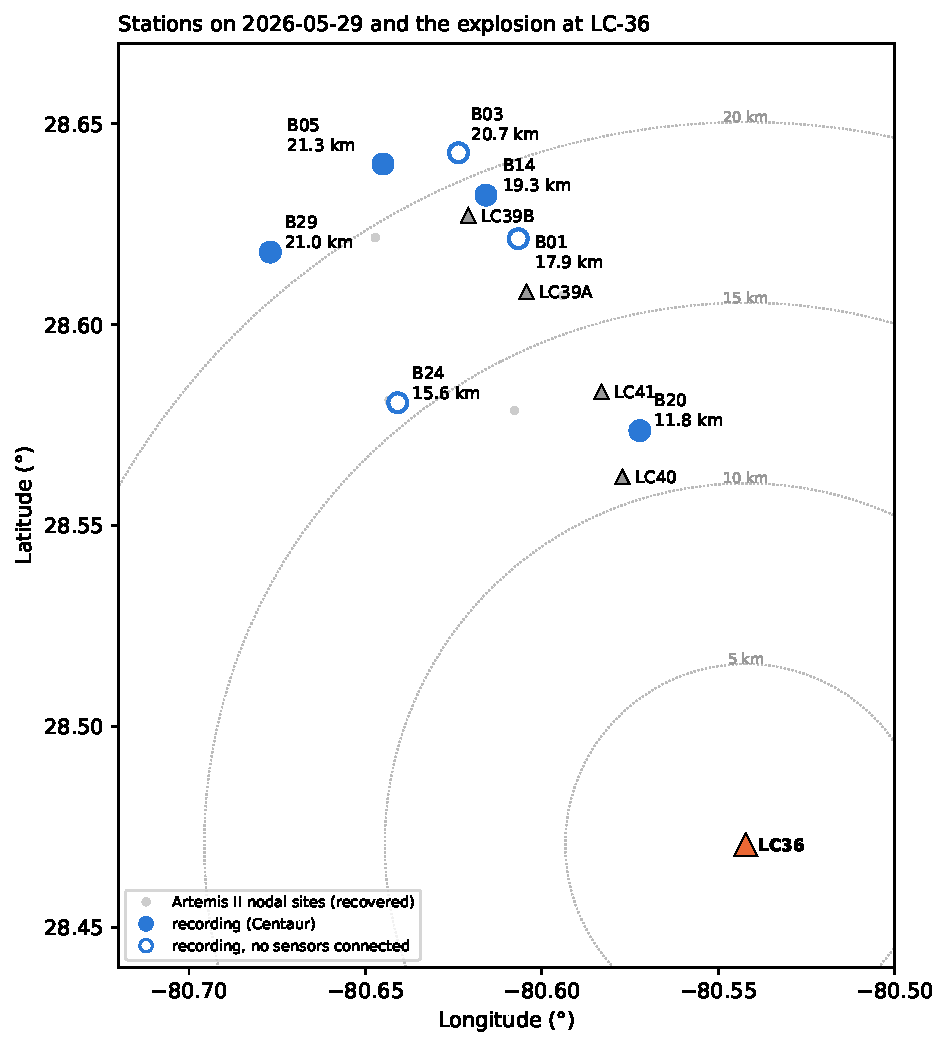
\includegraphics[width=0.62\textwidth]{station_map}
  \caption{Stations recording on 29~May~2026 (circles; open: digitizer
    recording but no sensors connected) and launch complexes (triangles).
    The explosion was at LC-36. Dotted circles: distance from LC-36.
    Grey dots: Artemis~II nodal sites, recovered in April.}
  \label{fig:map}
\end{figure}

\begin{table}[htbp]
  \centering
  \caption{Stations, distances and azimuths from LC-36, and channel status
    for the explosion (coordinates in \supptab{1}, channel-by-channel status in \supptab{2}).}
  \label{tab:stations}
  \small
  \begin{tabular}{lrrp{0.55	extwidth}}
\toprule
Station & Distance (km) & Azimuth ($^{\circ}$) & Working channels \\
\midrule
B20 & 11.79 & 345.6 & infraBSU DD1; Trillium (noisy; horizontals identical); Chaparral (clipped, faulty) \\
B24 & 15.55 & 321.6 & none (no sensors connected) \\
B01 & 17.87 & 339.3 & none (no sensors connected) \\
B14 & 19.31 & 338.1 & infraBSUs DD0, DD1, DD2; Trillium \\
B03 & 20.68 & 337.4 & none (no sensors; Centaur faulty) \\
B29 & 21.00 & 321.1 & infraBSU DD0; Trillium \\
B05 & 21.30 & 331.8 & infraBSU DD0; Trillium (DH2 at its stop) \\
\bottomrule
\end{tabular}

\end{table}

\subsection{Processing}

Waveforms were read from the network's SeisComP Data Structure archive
and corrected to pressure and ground velocity with the response of each
station's Centaur at the time, with the infraBSU sensor stage
(\SI{46}{\micro\volt\per\pascal}) prepended to the infrasound channels.
The Centaur at B14 wrote no response file between January and
14~June~2026; we used its first later file, whose settings are identical
to those of B01 two days before the explosion. Processing used ObsPy
\citep{Beyreuther2010,krischer_obspy_2015}, FlovoPy
\citep{flovopy_2026} and a shared library for the KSC papers
(\texttt{ksclib}; Data and Code Availability).

%% ============================================================
\section{Channel Status and Instrument Problems}
\label{sec:status}

An unattended network records whatever is connected to it. The
explosion, a large and well-located signal on every channel, is a
stringent test of what was.

\paragraph{Disconnected sensors.} B01, B03 and B24 recorded only
digitizer noise on all six channels: about \NGdeadDH~counts rms on the
seismometer inputs and \NGdeadDD~counts on the infrasound inputs, with flat
spectra and no microseism peak, two to five orders of magnitude below
the connected inputs (Figure~\ref{fig:dead}). Small airwave-timed
excursions of a few hundred counts appear on these inputs, as they do on
unconnected inputs at working stations (B20 HD2; CD1 and CD2 at B05 and
B29). With no sensor attached they are most likely pressure or vibration
acting on the digitizer and cabling.

\begin{figure}[htbp]
  \centering
  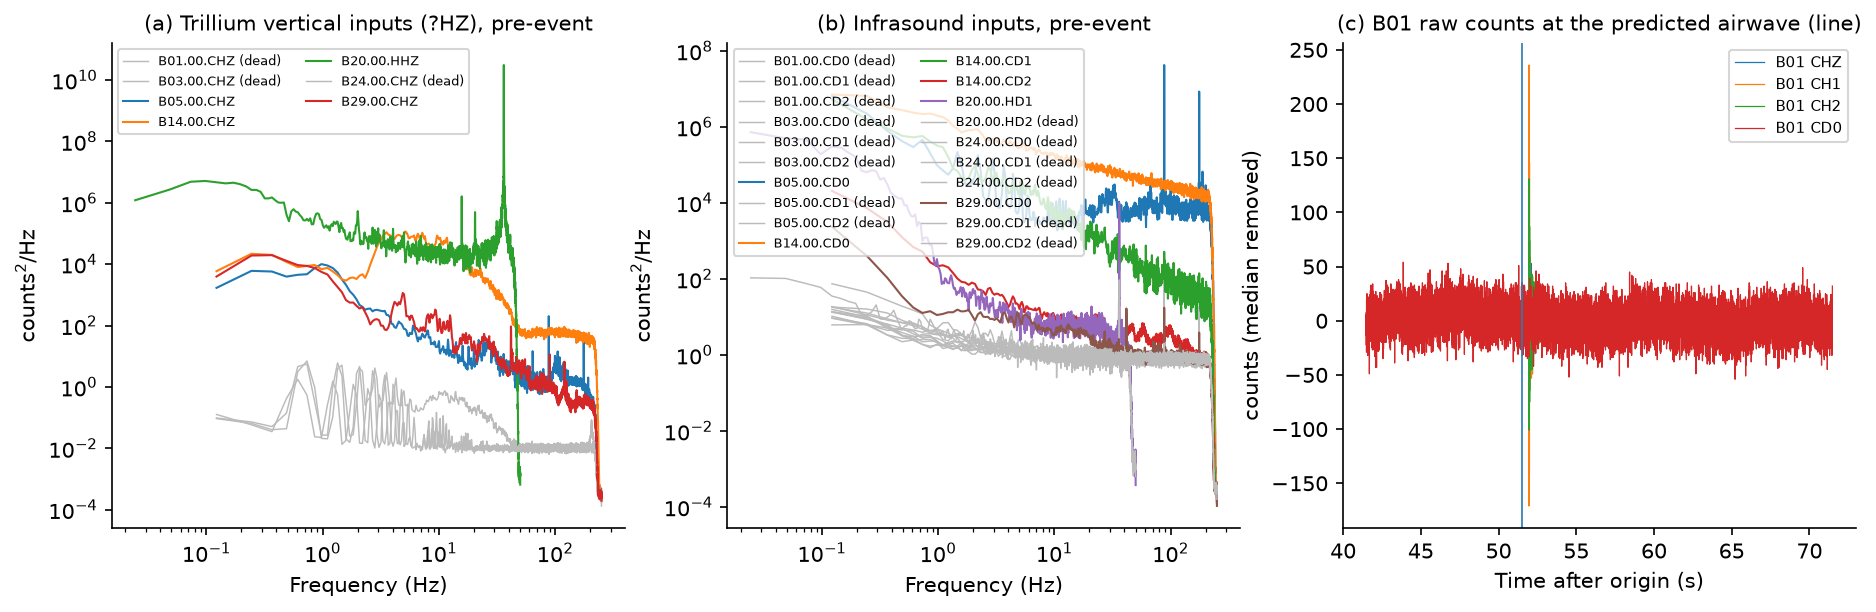
\includegraphics[width=\textwidth]{dead_station_evidence}
  \caption{Evidence for the disconnected sensors. (a,b)~Pre-event noise
    spectra, in raw counts, of the seismometer and infrasound inputs;
    inputs without sensors (grey) are flat, at the digitizer's own level.
    (c)~Raw counts at B01 around the predicted airwave arrival (line).}
  \label{fig:dead}
\end{figure}

\paragraph{Reversed infrasound polarity.} A blast wave begins with a
compression. B14 CD1, B14 CD2 and B05 CD0 begin with a rarefaction, and
B14 CD1 and CD2 are mirror images of the co-located CD0 (correlation
$\NGpolCorr$). The likely cause is a capillary tube fitted to the inner
rather than the outer nipple of the sensor. We reverse these channels
throughout.

\paragraph{Sensor-to-sensor differences.} The three infraBSUs at B14 sat
in the same tote. CD1 and CD2 record the airwave identically (coherence
at least 0.98 from 0.5 to \NGbCohHz~Hz), with a constant amplitude ratio
CD2/CD1~=~\NGbRatio{} below 40~Hz, a relative calibration difference of \NGbCal\%.
Above 100~Hz their ratio rises to $\NGresPeakDb$~dB near \NGresPeakHz~Hz and falls to
$\NGresMinDb$~dB near \NGresMinHz~Hz, a resonance of one sensor's inlet that the other
lacks (\suppfig{1}). Their noise levels above 0.5~Hz differ by almost
two orders of magnitude (\NGnoiseDDzero, \NGnoiseDDone{} and \NGnoiseDDtwo~Pa rms for CD0, CD1 and CD2).
Because the three shared one tote, none of these differences is a tote
effect; they lie in each sensor's inlet or electronics. The peak
pressures below are therefore uncertain by up to $\sim$\NGbCal\% until the
relative calibrations from the Artemis~II comparison
\citep{thompson_artemis2_recording_2026} are applied.

\paragraph{The B20 Chaparral.} The M25 clipped at the digitizer's
24-bit rail in \NGclipN{} intervals between the shock (\NGclipStart~s after the origin)
and \NGclipEnd~s (\suppfig{2}). It shares Centaur Sensor~B and its filters with
the co-located infraBSU, so the ratio of their raw counts in a band where
both are flat gives its sensitivity directly. Over \NGchapWindows{} coherent,
unclipped windows after \NGchapLaunches{} launches in 2026 (Figure~\ref{fig:chaparral}; \supptab{12}),
it was \NGchapEarly~V~Pa$^{-1}$ from January to 4~April and
\NGchapLate~V~Pa$^{-1}$ from 14~June to September, matching its nominal
0.4~V~Pa$^{-1}$. Between the field visits of 4~April and 14~June,
however, its apparent sensitivity jumped between $\sim$\NGchapFaultA,
$\sim$\NGchapFaultB{} and \NGchapFaultC~V~Pa$^{-1}$, and rose within single events as
the signal decayed. At the explosion it read about \NGchapExplosion~V~Pa$^{-1}$.
The sensor was faulty or mis-set during that interval, and we do not use
it.

\begin{figure}[htbp]
  \centering
  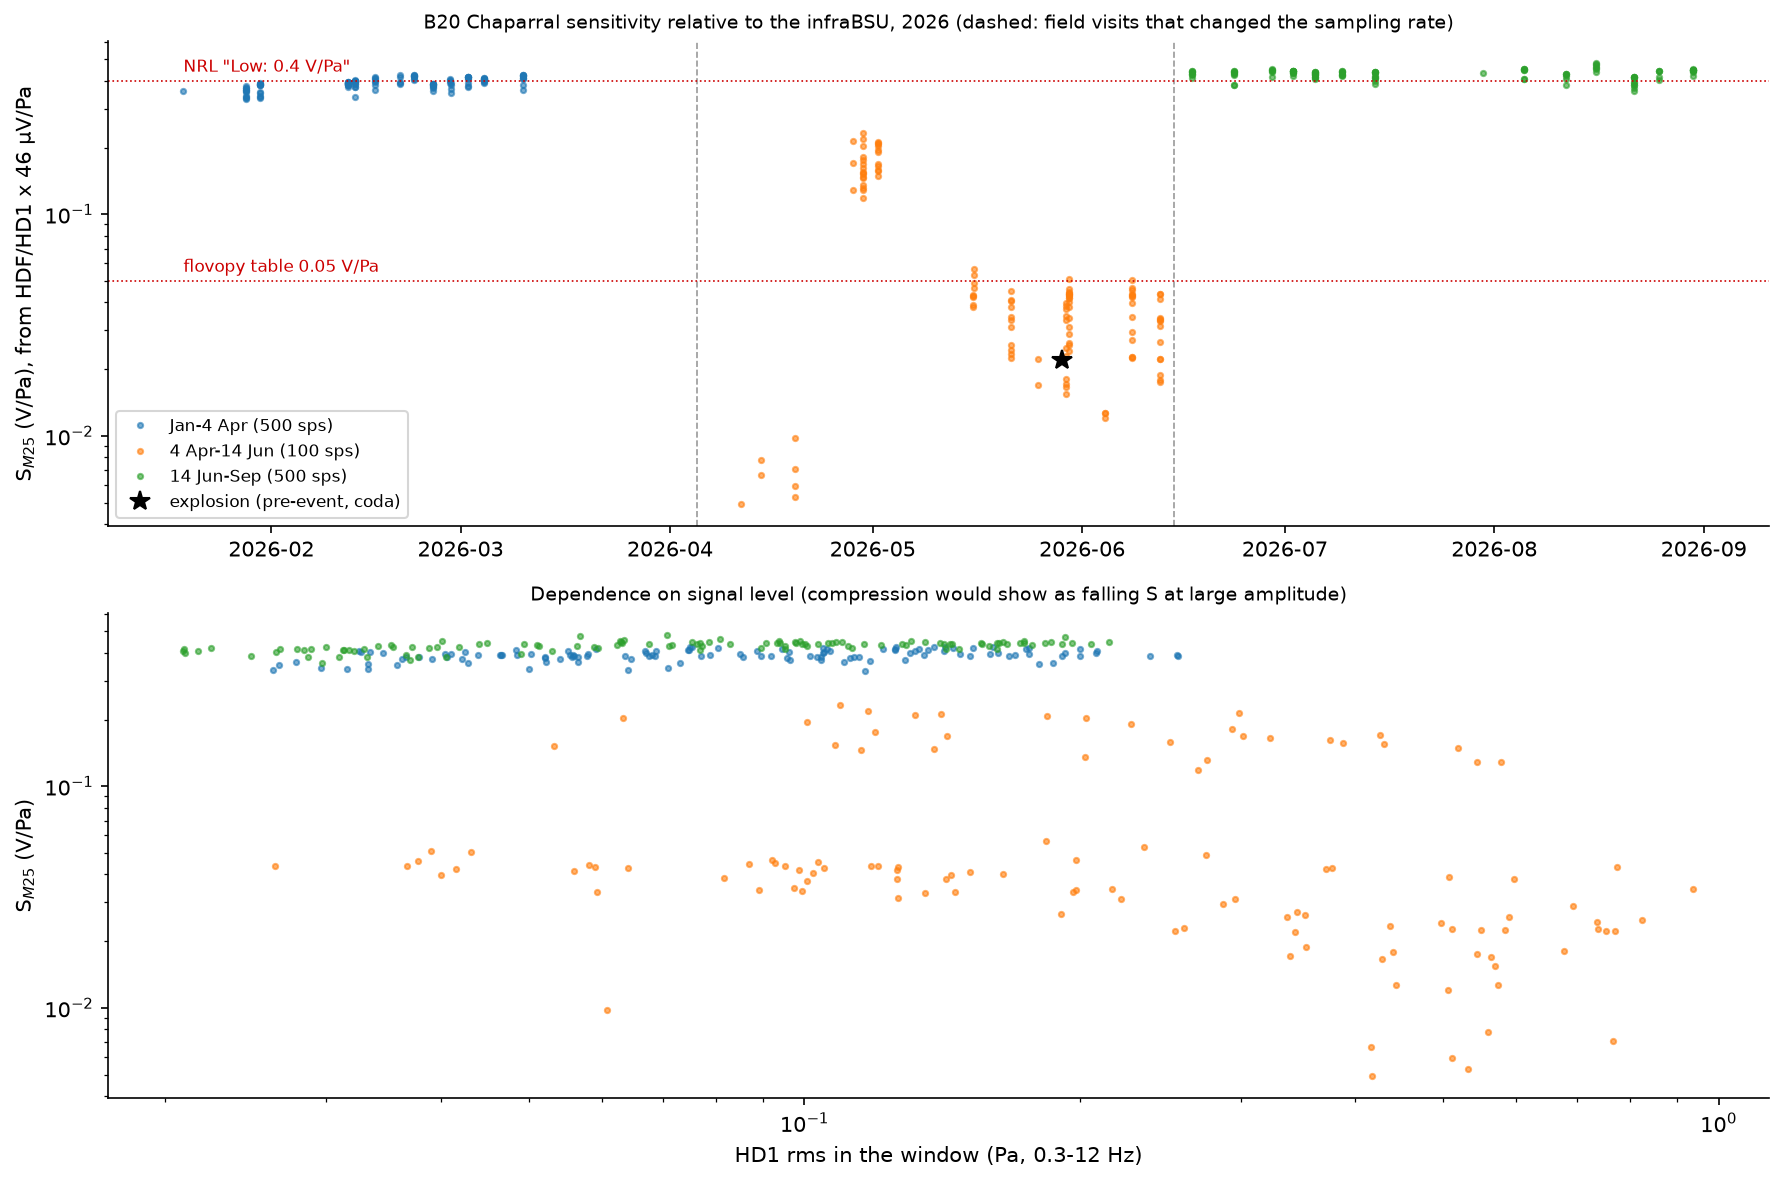
\includegraphics[width=\textwidth]{chaparral_sensitivity}
  \caption{Sensitivity of the B20 Chaparral M25 relative to the
    co-located infraBSU through 2026, from coherent, unclipped windows
    after launches and around the explosion (star). Dashed lines: field
    visits. (b)~Dependence on signal level.}
  \label{fig:chaparral}
\end{figure}

\paragraph{The B20 Trillium.} Its two horizontal channels correlate at
\NGbtwentyCorr{} or more on every day sampled from February to August, so they record one
signal twice. Its vertical is dominated by tones near 15 and 35~Hz from
nearby machinery, and its air-to-ground coupling has the opposite sign to
every other site (Section~\ref{sec:coupling}). We use B20's vertical only
where noted, and treat its polarity as uncertain.

\paragraph{Sampling rate.} B20 recorded at 100~samples~s$^{-1}$. Low-pass
filtering and decimating the 500~samples~s$^{-1}$ records to
100~samples~s$^{-1}$ lowers the B14 peaks by \NGdecBfourteen\% (B14's shock front
is very steep), but those at B29 and B05 by only \NGdecOther\%; impulse and
duration change by less than \NGdecImpDur\%.

The working channels are therefore infraBSUs at B20 (HD1, \NGdistBtwenty~km), B14
(CD0--CD2, \NGdistBfourteen~km), B29 (CD0, \NGdistBtwentynine~km) and B05 (CD0, \NGdistBzerofive~km), and
seismometers at B14, B29 and B05 (and B20's vertical).

%% ============================================================
\section{Overview of the Recordings and Origin Time}

The airwave is a sharp N-like pulse at every station, followed by a
coda of several seconds (Figure~\ref{fig:overview}a). Vertical ground
velocity peaks with the airwave, but at B14, B29 and B05 a weaker,
dispersed seismic wavetrain begins within 10~s of the origin, tens of
seconds before the airwave (Figure~\ref{fig:overview}b). The airwave is
very broadband: its power exceeds the noise tenfold from \NGsnrLow{} to \NGsnrHigh~Hz at
the quieter infraBSUs (\suppfig{3}), but \NGenergyLow\% of its energy lies
below 5~Hz.

\begin{figure*}[htbp]
  \centering
  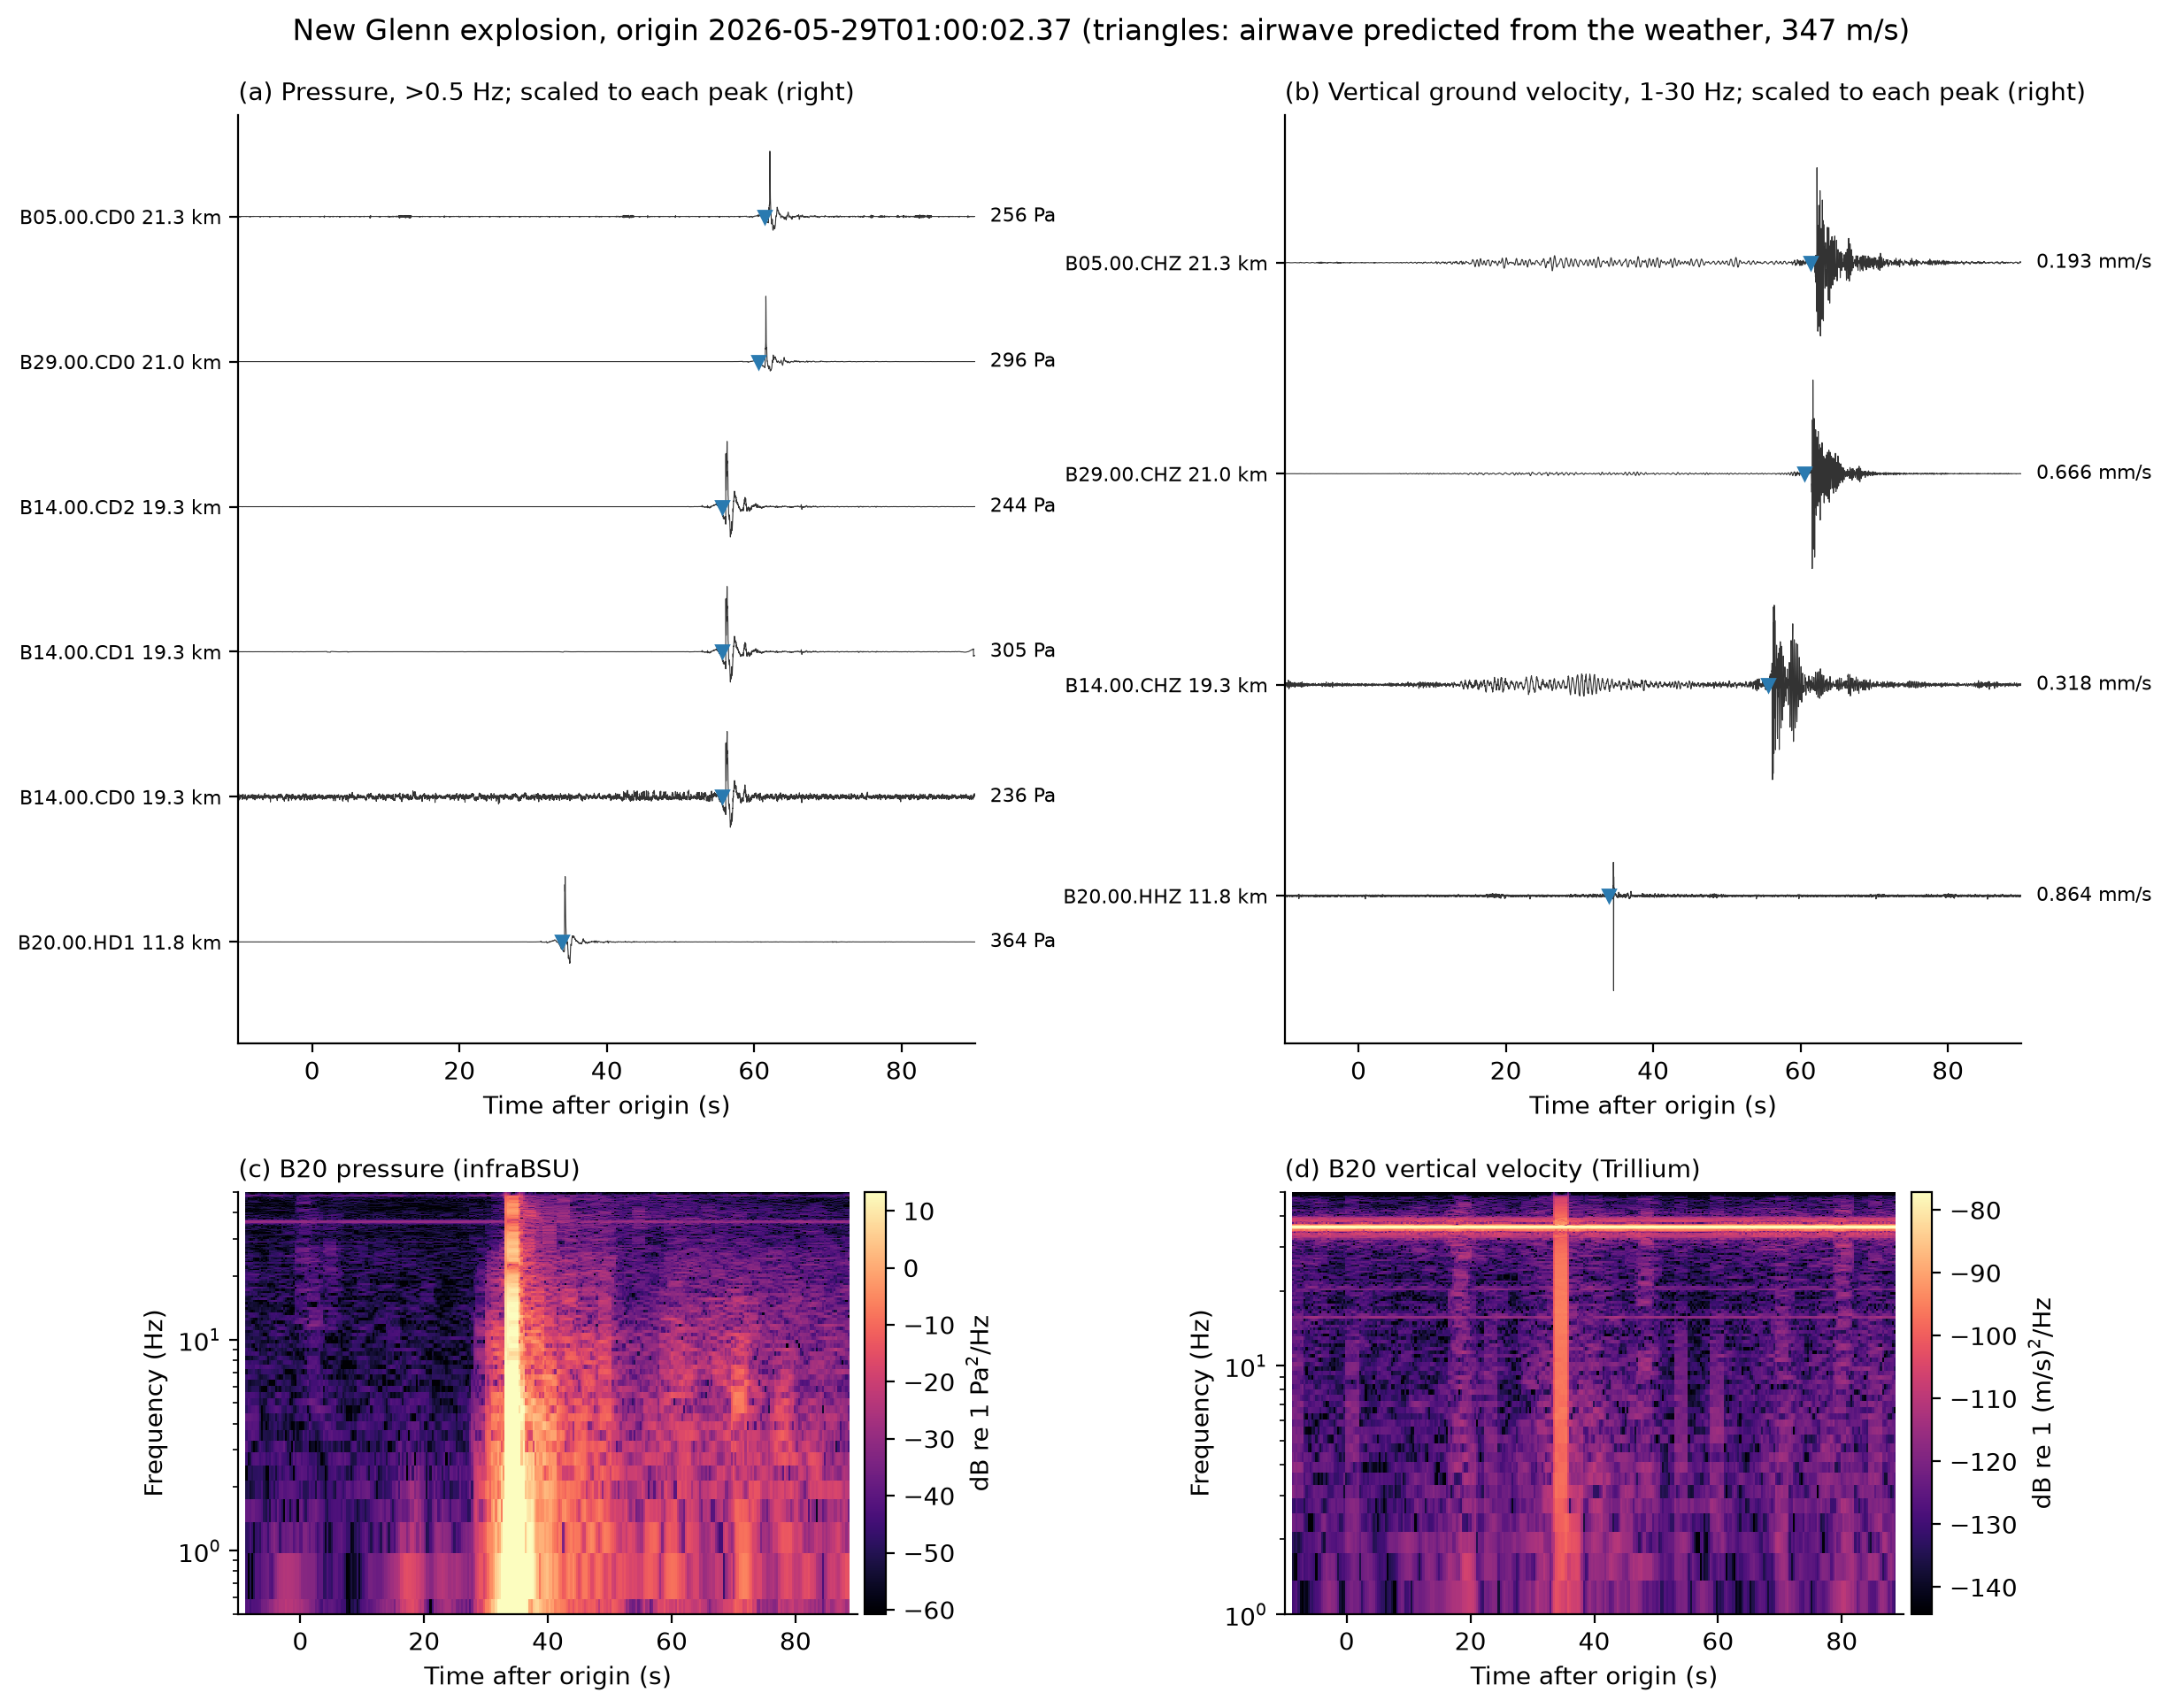
\includegraphics[width=\textwidth]{data_overview}
  \caption{Record sections of (a)~pressure ($>$0.5~Hz) and (b)~vertical
    ground velocity (1--30~Hz), sorted by distance and scaled to each
    trace's peak (right). Triangles: airwave arrival predicted from the
    weather. (c,d)~Spectrograms at B20.}
  \label{fig:overview}
\end{figure*}

The origin time was not known to the second. We take the airwave onset
at each working infraBSU as the first sample above 5\% of the peak (and
above five times the noise), and the speed of sound from surface weather
at the Cape Canaveral Skid Strip (XMR, 2~km from LC-36) and the Shuttle
Landing Facility (TTS, within the network) within 30~minutes of the event
\citep{iem_asos}: \NGtemp~$^{\circ}$C, \NGrh\% relative humidity, \NGpressure~hPa and
a \NGwind~m~s$^{-1}$ wind from \NGwindFrom$^{\circ}$. The still-air sound speed
\citep{cramer1993} is \NGczero~m~s$^{-1}$, and the wind is a
\NGheadwind~m~s$^{-1}$ headwind on every ray, giving
\NGceff~m~s$^{-1}$. The six onsets then give an origin of
\NGoriginPrecise~UTC with a station spread of \NGoriginSpread~s (Figure~\ref{fig:origin}; \supptab{3}--\supptab{6}).
Other onset definitions and weather choices give \NGoriginRange, and a
fit with the speed left free gives \NGoriginFree{} at \NGspeedFree~m~s$^{-1}$: the far
stations are slightly late relative to the surface weather.

The KSC weather towers \citep{ksc_wxarchive} test the surface weather
along the paths themselves (\suppfig{8}). Between 00:50 and 01:10~UTC,
\NGtowerN{} towers around the paths recorded 6~ft (2~m)
temperatures of \NGtowerTcoast~$^{\circ}$C near the pad and
\NGtowerTinland~$^{\circ}$C near the stations, with 204~ft (62~m) within
\NGtowerDTmax~$^{\circ}$C of 6~ft: no surface inversion at tower heights. The
wind, from the west-north-west, strengthened with height, from a
\NGtowerHeadLow~m~s$^{-1}$ headwind along the paths at 12~ft to
\NGtowerHeadHigh~m~s$^{-1}$ at 204~ft. Interpolating the towers along each path
gives \NGtowerCpathLow~m~s$^{-1}$ at 6--54~ft and an origin within
\NGtowerShiftLow~s of that from the airport stations. With the 204~ft towers
the speed falls to \NGtowerCpathHigh~m~s$^{-1}$, the origin moves
\NGtowerShiftHigh~s \NGtowerShiftHighDir{} and the station spread falls to
\NGtowerSpreadHigh~s, so the wind above 10~m probably contributes to the late
far stations; the free-fit speed is lower still. No balloon sounding was
made within 13~h of the explosion. We adopt \NGorigin~$\pm$~1~s.

This origin assumes that the airwave travels at the speed of sound all
the way from the pad. Near the pad, however, the blast front is a shock
that moves faster than sound. Integrating the excess speed along each
ray with the normal-shock Mach number, as for AMOS-6
\citep{thompson_amos6_2026}, the front reaches the stations
\NGadvanceSph~s earlier than a sound wave would if each station's peak
overpressure is extrapolated inward by spherical spreading to 10~m, and
\NGadvance~s earlier with the Kinney--Graham overpressure for the yield of
Section~\ref{sec:yield} \citep{kinney1985}. Spherical spreading
underestimates the pressure close to the source, so the first is a lower
bound. Allowing for the advance moves the origin to
\NGoriginCorrRange~UTC: about \NGfireballGap~s after the first fireball seen on
video and \NGflashGapRange~s before the main flash
\citep{silber_scamfer_newglenn_2026}, which is within our uncertainty.
The video's clock is the weaker link: the footage is identified only in
their supplement, and the accuracy of its timestamp is not stated.
The airwave we record therefore comes from the main flash. An origin at
the first fireball, \NGflashFireballSep~s earlier, would need an airwave far
faster than the \NGceff~m~s$^{-1}$ that the weather gives. The pad position
adds a smaller uncertainty: with the coordinates of
\citet{silber_scamfer_newglenn_2026} the origin would move \NGpadShift~s
\NGpadShiftDir.

\begin{figure}[htbp]
  \centering
  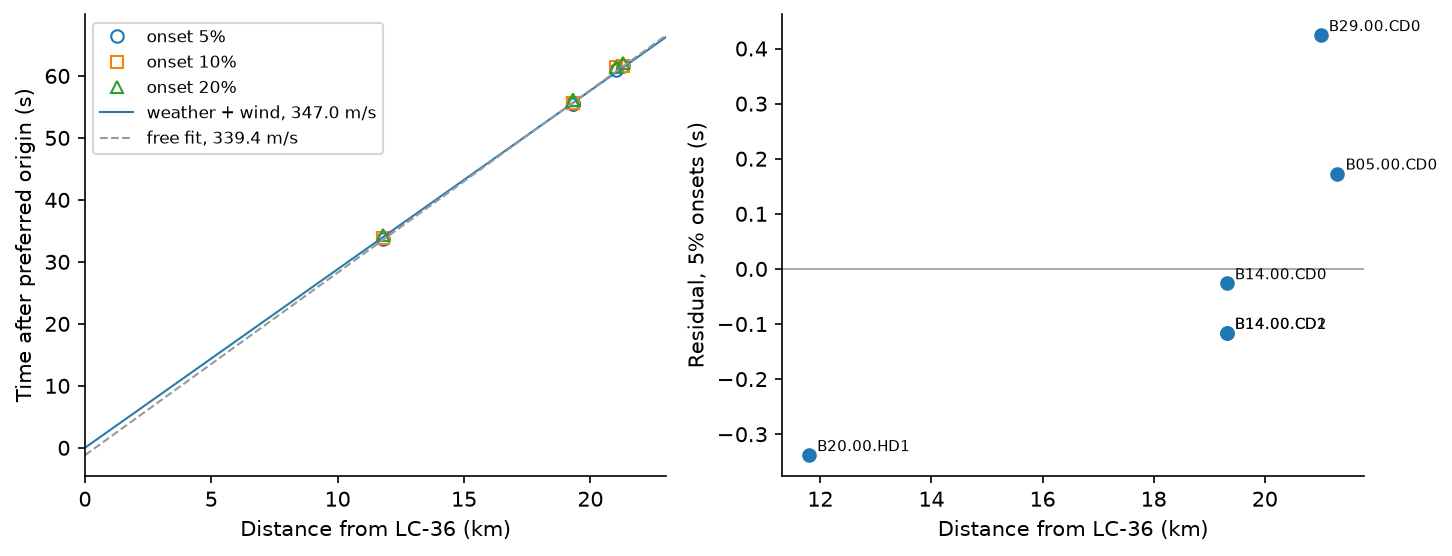
\includegraphics[width=\textwidth]{origin_time}
  \caption{Airwave onsets against distance after the preferred origin,
    with the weather-based (solid) and free-speed (dashed) fits, and the
    residuals of the 5\% onsets.}
  \label{fig:origin}
\end{figure}

%% ============================================================
\section{The Blast Wave}

\subsection{Amplitudes and decay with distance}

Positive peak overpressures (high-passed at 0.05~Hz) are \NGpBtwenty~Pa at B20,
\NGpFar~Pa across the three sensors at B14, \NGpBtwentynine~Pa at B29 and \NGpBzerofive~Pa at
B05 (Table~\ref{tab:blast}; \supptab{7}). Positive phases last \NGtpos~s and carry
impulses of \NGipos~Pa~s; negative phases are three to seven times weaker
than positive ones (\suppfig{4}).

\begin{table}[htbp]
  \centering
  \caption{Blast-wave parameters ($>$0.05~Hz). B14: range over its three
    infraBSUs.}
  \label{tab:blast}
  \begin{tabular}{lrrrrr}
\toprule
Station & $r$ (km) & $P_+$ (Pa) & $P_-$ (Pa) & $t_+$ (s) & $I_+$ (Pa~s) \\
\midrule
B20 & 11.8 & 407 & $-125$ & 0.44 & 61 \\
B14 & 19.3 & 264--342 & $-86$ to $-111$ & 0.38 & 42--54 \\
B29 & 21.0 & 315 & $-43$ & 0.36 & 28 \\
B05 & 21.3 & 273 & $-61$ & 0.37 & 30 \\
\bottomrule
\end{tabular}

\end{table}

Peak pressure falls only as $r^{-\NGnPeak}$ between \NGdistBtwenty{} and
\NGdistBzerofive~km (Figure~\ref{fig:amp}). Splitting the band shows why: below 4~Hz
the peak falls as $r^{-\NGnLow}$, close to spherical spreading,
whereas above 4~Hz it hardly falls at all (\supptab{8}). Positive impulse, dominated
by the low frequencies, falls as $r^{-\NGnImp}$, and $I_+ r$ is
\NGiposr~Pa~s~km at every station. Pressure spectra reduced to 1~km by
spherical spreading and ISO~9613-1 absorption \citep{iso9613_1} agree within
a spread of about \NGredLow~dB below 4~Hz, but spread by about \NGredHigh~dB above it
(\suppfig{5}). The slow decay of the peak is therefore carried by the
higher frequencies. Two effects may contribute: B20's 100~samples~s$^{-1}$,
which may under-record its peak by up to $\sim$\NGdecMax\% (if so, the peak
decays as $r^{-\NGnPeakCorr}$), and night-time refraction, which can favour the
higher frequencies at the far stations. The positive-phase duration also
shortens slightly with distance, which weak-shock theory does not
predict; propagation modelling is needed.

\begin{figure*}[htbp]
  \centering
  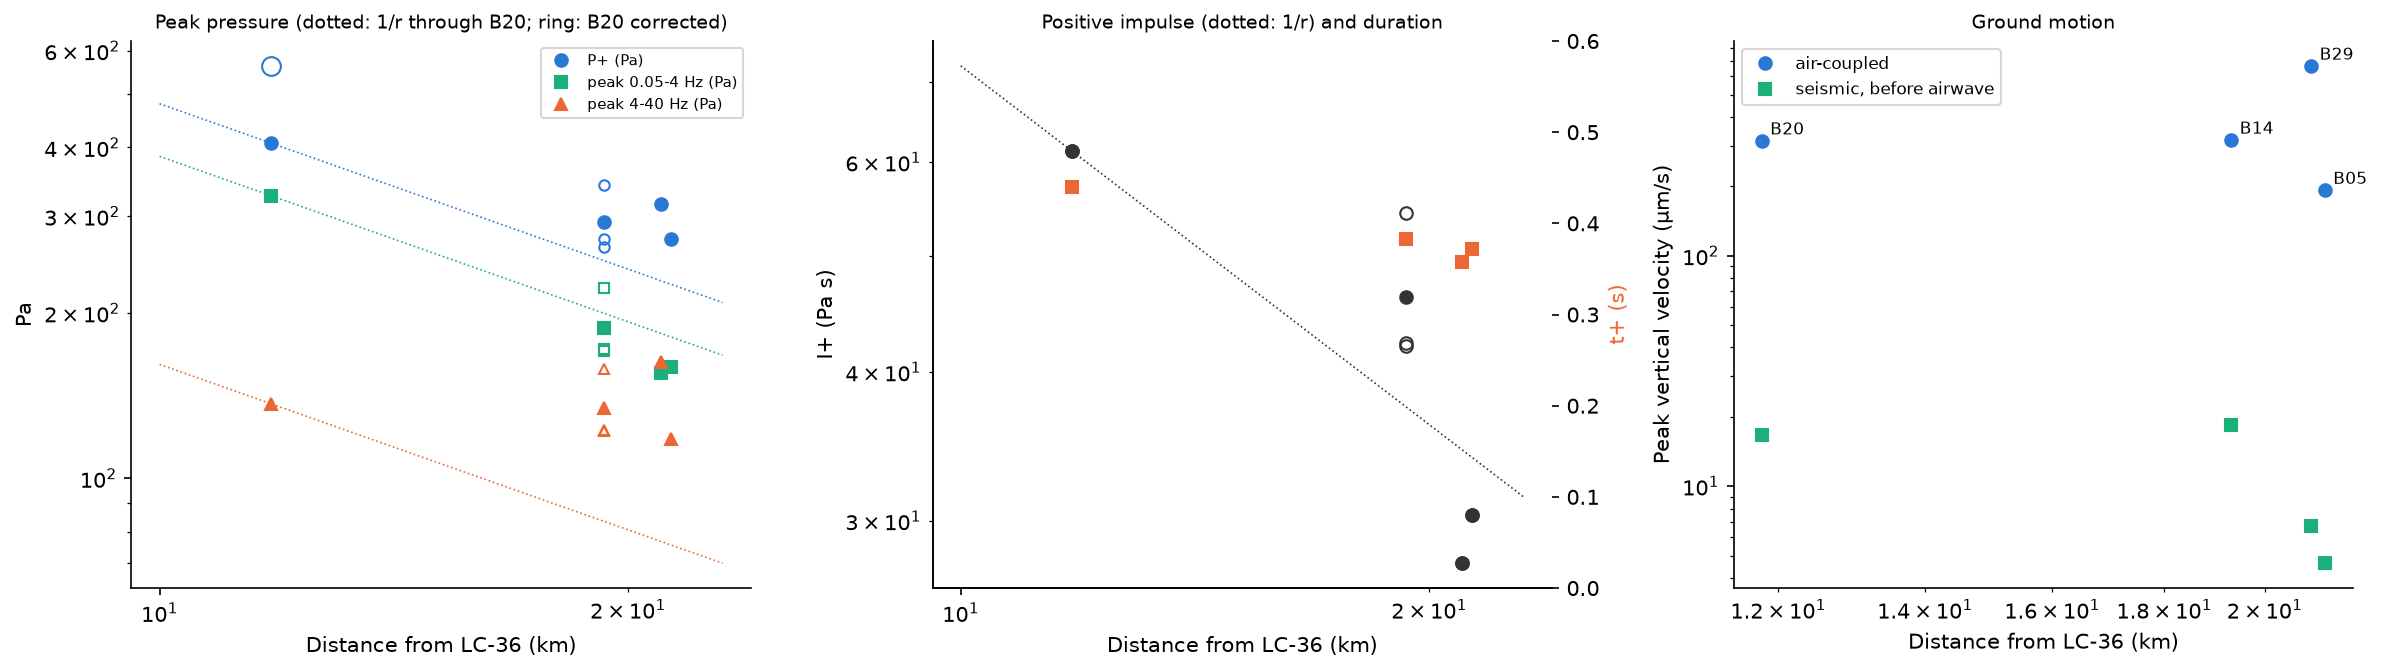
\includegraphics[width=\textwidth]{amplitude_vs_distance}
  \caption{(a)~Peak pressure, broadband and in two bands, against
    distance (open symbols: individual B14 sensors; ring: B20 corrected
    for decimation; dotted: $1/r$). (b)~Positive impulse and duration.
    (c)~Peak vertical velocity of the air-coupled motion and of the
    seismic waves ahead of the airwave.}
  \label{fig:amp}
\end{figure*}

\subsection{Yield}
\label{sec:yield}

The Kinney--Graham relations for TNT \citep{kinney1985}, treating the
explosion as a surface burst (twice the free-air yield), give a TNT
equivalent of about \NGyieldP~t from the peak overpressures (\NGyieldPrange~t across
the six sensors) and about \NGyieldT~t from the positive-phase durations
(\NGyieldTrange~t). The estimate from peak overpressure agrees closely with
the 131~t (0.131~kt) of \citet{silber_scamfer_newglenn_2026}, derived
from infrasound at regional and continental distances. The longer
positive phase is consistent with a propellant explosion, which releases
energy more slowly than TNT and so produces a longer, weaker pulse. Both
estimates rest on relations fitted at much smaller scaled distances (here
$Z \approx{}$\NGzRange~m~kg$^{-1/3}$) and on uncalibrated relative
sensitivities, so we regard the agreement as confirming a yield of
order 100--200~t rather than refining it.

%% ============================================================
\section{Air-to-Ground Coupling}
\label{sec:coupling}

At each site with an infraBSU and a Trillium, the airwave presses the
ground down as it passes. Vertical displacement follows pressure with no
little or no lag ($\leq$\NGlagMax~s; Figure~\ref{fig:coupling}): the
correlation is $\NGcorrBfourteen$ at B14 (all three sensors), $\NGcorrBtwentynine$ at B29 and
$\NGcorrBzerofive$ at B05, with the sign expected for loading. Vertical velocity
therefore follows $-C\,\mathrm{d}p/\mathrm{d}t$, where $C$ is the
compliance, which is why regressing velocity on pressure, as for
Artemis~II and AMOS-6 \citep{thompson_amos6_2026}, correlates poorly
here ($|r| = {}$\NGvpCorr). The compliance is $\NGcompBfourteen$~nm~Pa$^{-1}$ at B14
(\NGcompBfourteenRange{} across its sensors), $\NGcompBtwentynine$~nm~Pa$^{-1}$ at B29 and
$\NGcompBzerofive$~nm~Pa$^{-1}$ at B05 (\supptab{9}). Conventional coupling ratios are
\NGkRms~\si{\micro\metre\per\second\per\pascal} (rms) and
\NGkPeak~\si{\micro\metre\per\second\per\pascal} (peak) at 1--40~Hz, the
same order as the 2.31~\si{\micro\metre\per\second\per\pascal} found for
AMOS-6 at 1.4~km \citep{thompson_amos6_2026}.

\begin{figure}[htbp]
  \centering
  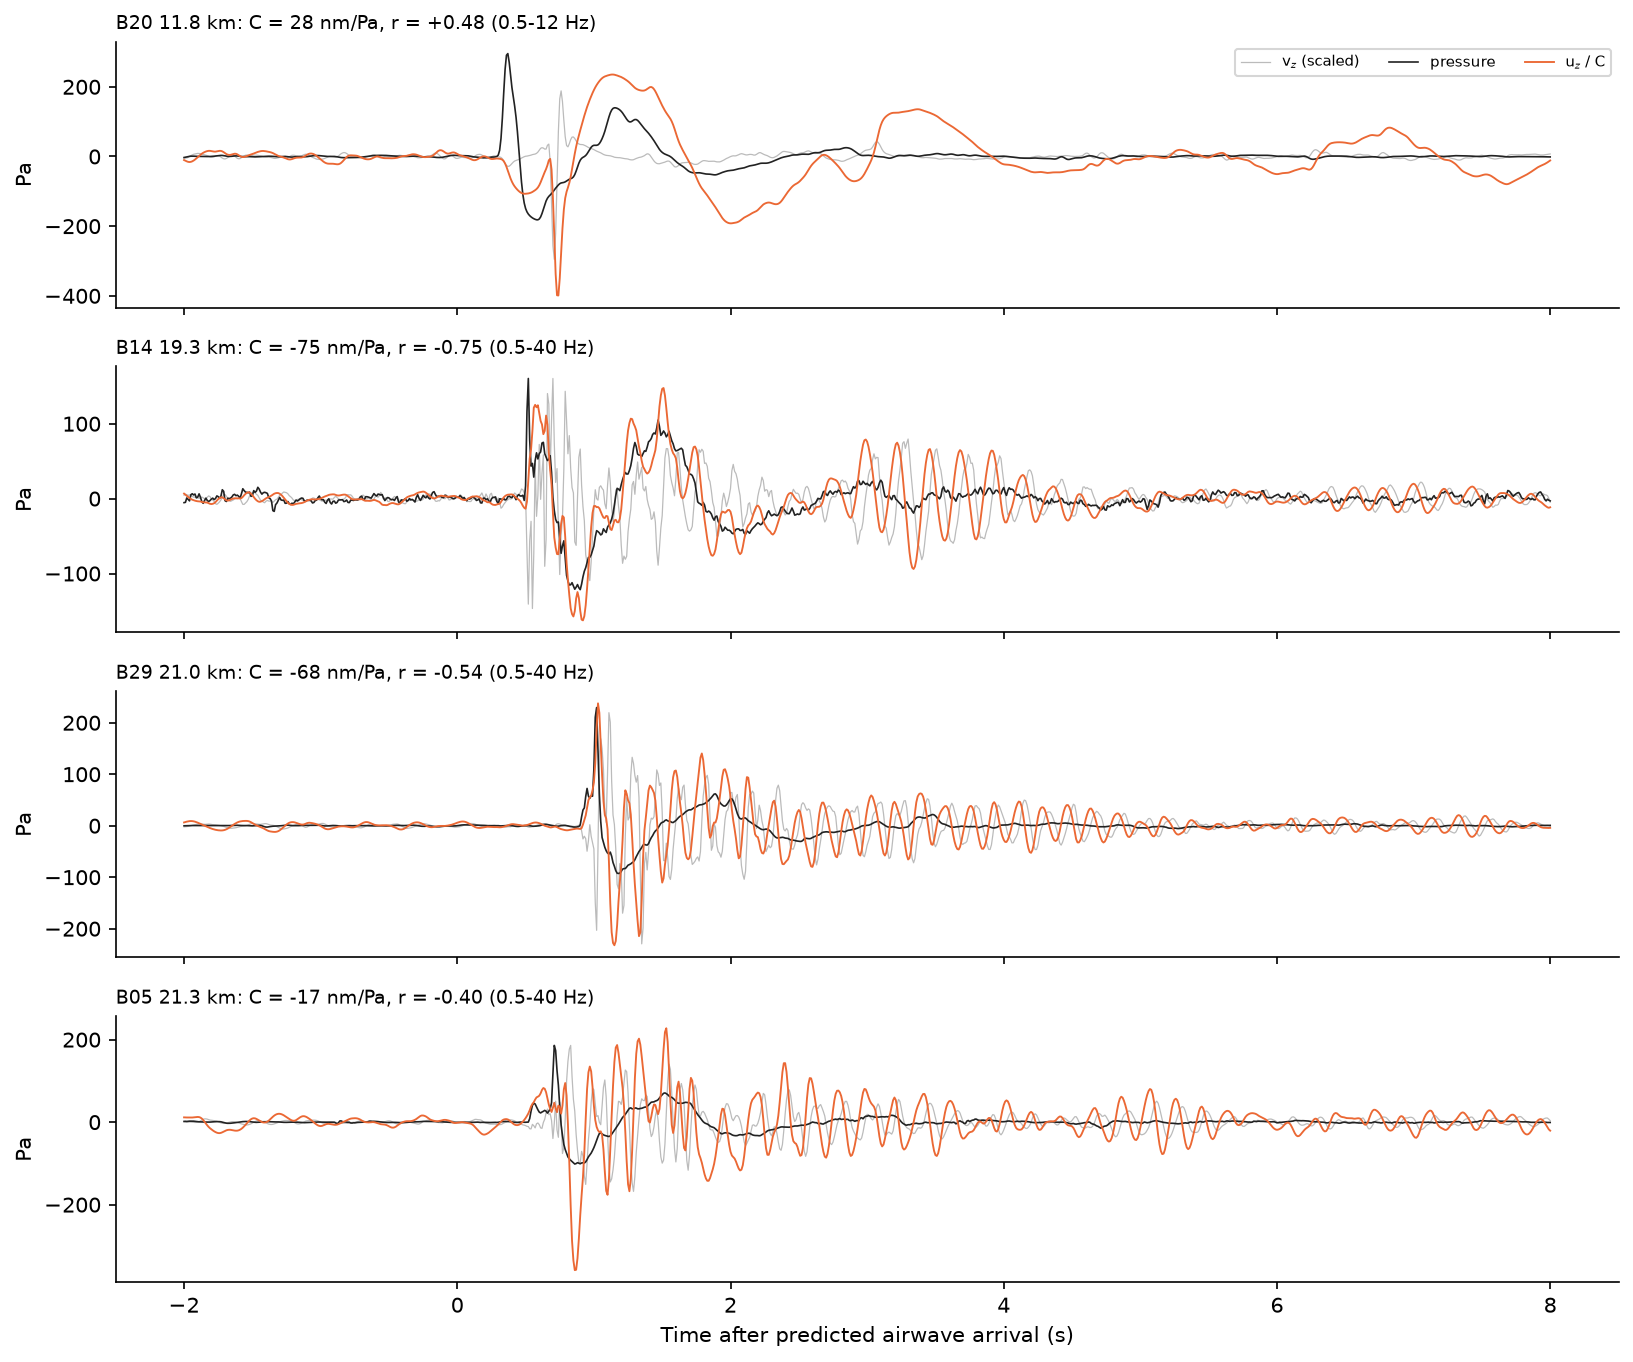
\includegraphics[width=\textwidth]{coupling_waveforms}
  \caption{Pressure (black) and vertical displacement divided by the
    fitted compliance (orange) at each site; vertical velocity (grey,
    scaled) for reference. Times after the predicted airwave arrival.}
  \label{fig:coupling}
\end{figure}

Applying the same code to the Artemis~II launch at the two sites
recorded by both events gives compliances of $\NGcompAtwoBzerofive$~nm~Pa$^{-1}$ at B05
and $\NGcompAtwoBtwentynine$~nm~Pa$^{-1}$ at B29, within \NGcompAgree\% of the explosion's values,
whereas the rms coupling ratios differ by a factor of two (B05: \NGkArtBzerofive{} and
\NGkNgBzerofive; B29: \NGkArtBtwentynine{} and \NGkNgBtwentynine~\si{\micro\metre\per\second\per\pascal}; \supptab{10}). The
coupling ratio depends on the source spectrum, but the compliance
describes the site.

The spectral compliance $|C(f)|$ is flat at \NGczeroRange~nm~Pa$^{-1}$ below
2.5~Hz (\NGczeroBzerofive~nm~Pa$^{-1}$ at B05), peaks near the frequency at which the
shock sets the ground ringing (\NGfzeroBfourteen~Hz at B14, \NGfzeroBtwentynine~Hz at B29, \NGfzeroBzerofive~Hz at
B05), and falls above $\sim$15~Hz (\suppfig{6}). This is not the
$1/f$ behaviour of a uniform half-space loaded by a moving pressure wave,
but resembles a soft layer over stiffer ground. The same 4--5~Hz band is
where the AMOS-6 transfer function peaked at BCHH
\citep{thompson_amos6_2026}. B20 is the exception: its compliance is
positive ($\NGcompBtwenty$~nm~Pa$^{-1}$, correlation $\NGcorrBtwenty$), which together with
its other problems (Section~\ref{sec:status}) suggests a reversed or
faulty vertical.

%% ============================================================
\section{Seismic Waves Ahead of the Airwave}

\subsection{Arrivals}

At B14, B29 and B05 the first seismic arrivals come \NGfirstArrival~s after the
origin (Figure~\ref{fig:seismic}), giving apparent velocities of
\NGvFirst~km~s$^{-1}$ (AIC picks in two bands, differing by \NGaicDiff~s
because the arrivals are emergent), \NGlead~s ahead of the airwave (\supptab{11}). A
long wavetrain follows, with most of its energy at 1--4~Hz and its
envelope peaking at \NGwavePeak~s (\NGwaveSpeed~km~s$^{-1}$), and lasts until
the airwave arrives. Its peak vertical velocity is \NGseisPeak~\si{\micro\metre\per\second},
\NGairOverSeis{} times smaller than the air-coupled motion. At B20 the noise is
\NGbtwentyNoise{} times higher than at B29 and B05, and only a burst at \NGbtwentyBurst~s
(\NGbtwentyBurstSpeed~km~s$^{-1}$) stands out.

\begin{figure*}[htbp]
  \centering
  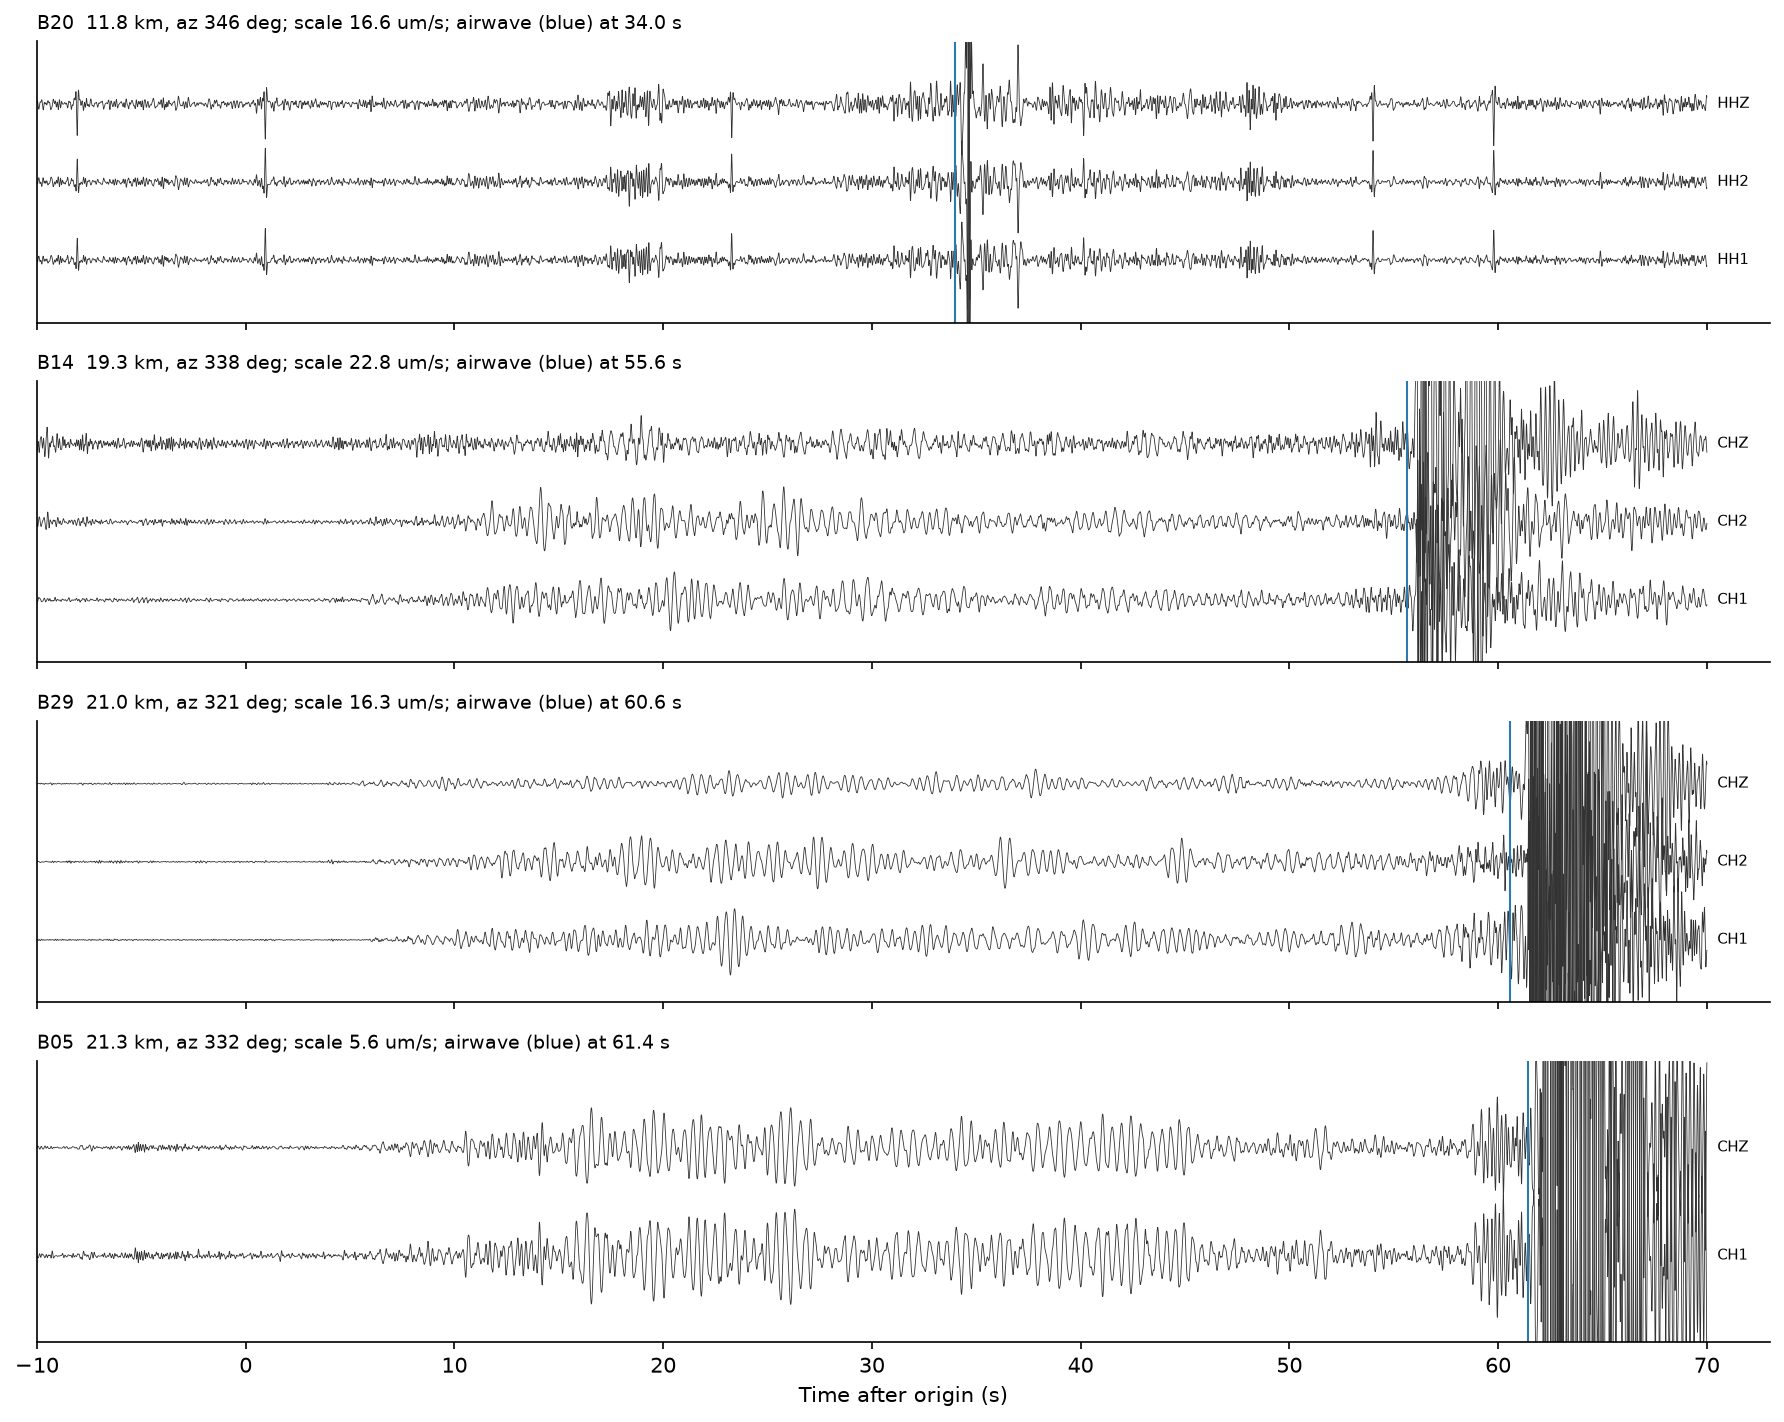
\includegraphics[width=\textwidth]{seismic_record_section}
  \caption{Three-component ground velocity (2--12~Hz) from the origin to
    just after the airwave (blue line), each station scaled to its
    largest seismic amplitude before the airwave.}
  \label{fig:seismic}
\end{figure*}

Our previous recordings at KSC did not show such a separation, for two
reasons: the stations were within a few kilometres of the source, and
launches are emergent. An impulsive source \NGdistRangeRound~km away separates the
two wavefields by tens of seconds.

\subsection{Dispersion}

Multiple-filter analysis of the verticals at B14, B29 and B05 gives a
fundamental-mode Rayleigh group velocity falling from \NGrayLowF~km~s$^{-1}$
at 0.5~Hz to \NGrayMid~km~s$^{-1}$ at 1.5--3~Hz
(Figure~\ref{fig:ftan}). The horizontals at B14 and B29 were rotated to
radial and transverse assuming the usual installation (CH1 north),
which the 1--3~Hz Rayleigh polarisation supports (CH1 at
\NGdhAz$^{\circ}$). With this orientation the radial dispersion matches
the vertical's, and the transverse shows a distinct Love-wave curve,
nearly identical at the two stations: \NGloveLowF~km~s$^{-1}$ at 0.5~Hz,
falling to \NGloveMin~km~s$^{-1}$ at \NGloveMinF~Hz. Above 1.8~Hz the transverse
ridge jumps to \NGloveHigh~km~s$^{-1}$, close to the first higher Love
mode of the models below. The Love waves are strong: the transverse
ridge is about \NGtOverR{} times the radial at 0.5--3~Hz. Along the
fundamental Rayleigh ridge the horizontal-to-vertical amplitude ratio
rises from about \NGhvLowF{} at 0.5~Hz to \NGhvPeak{} at \NGhvPeakF~Hz.

\begin{figure*}[htbp]
  \centering
  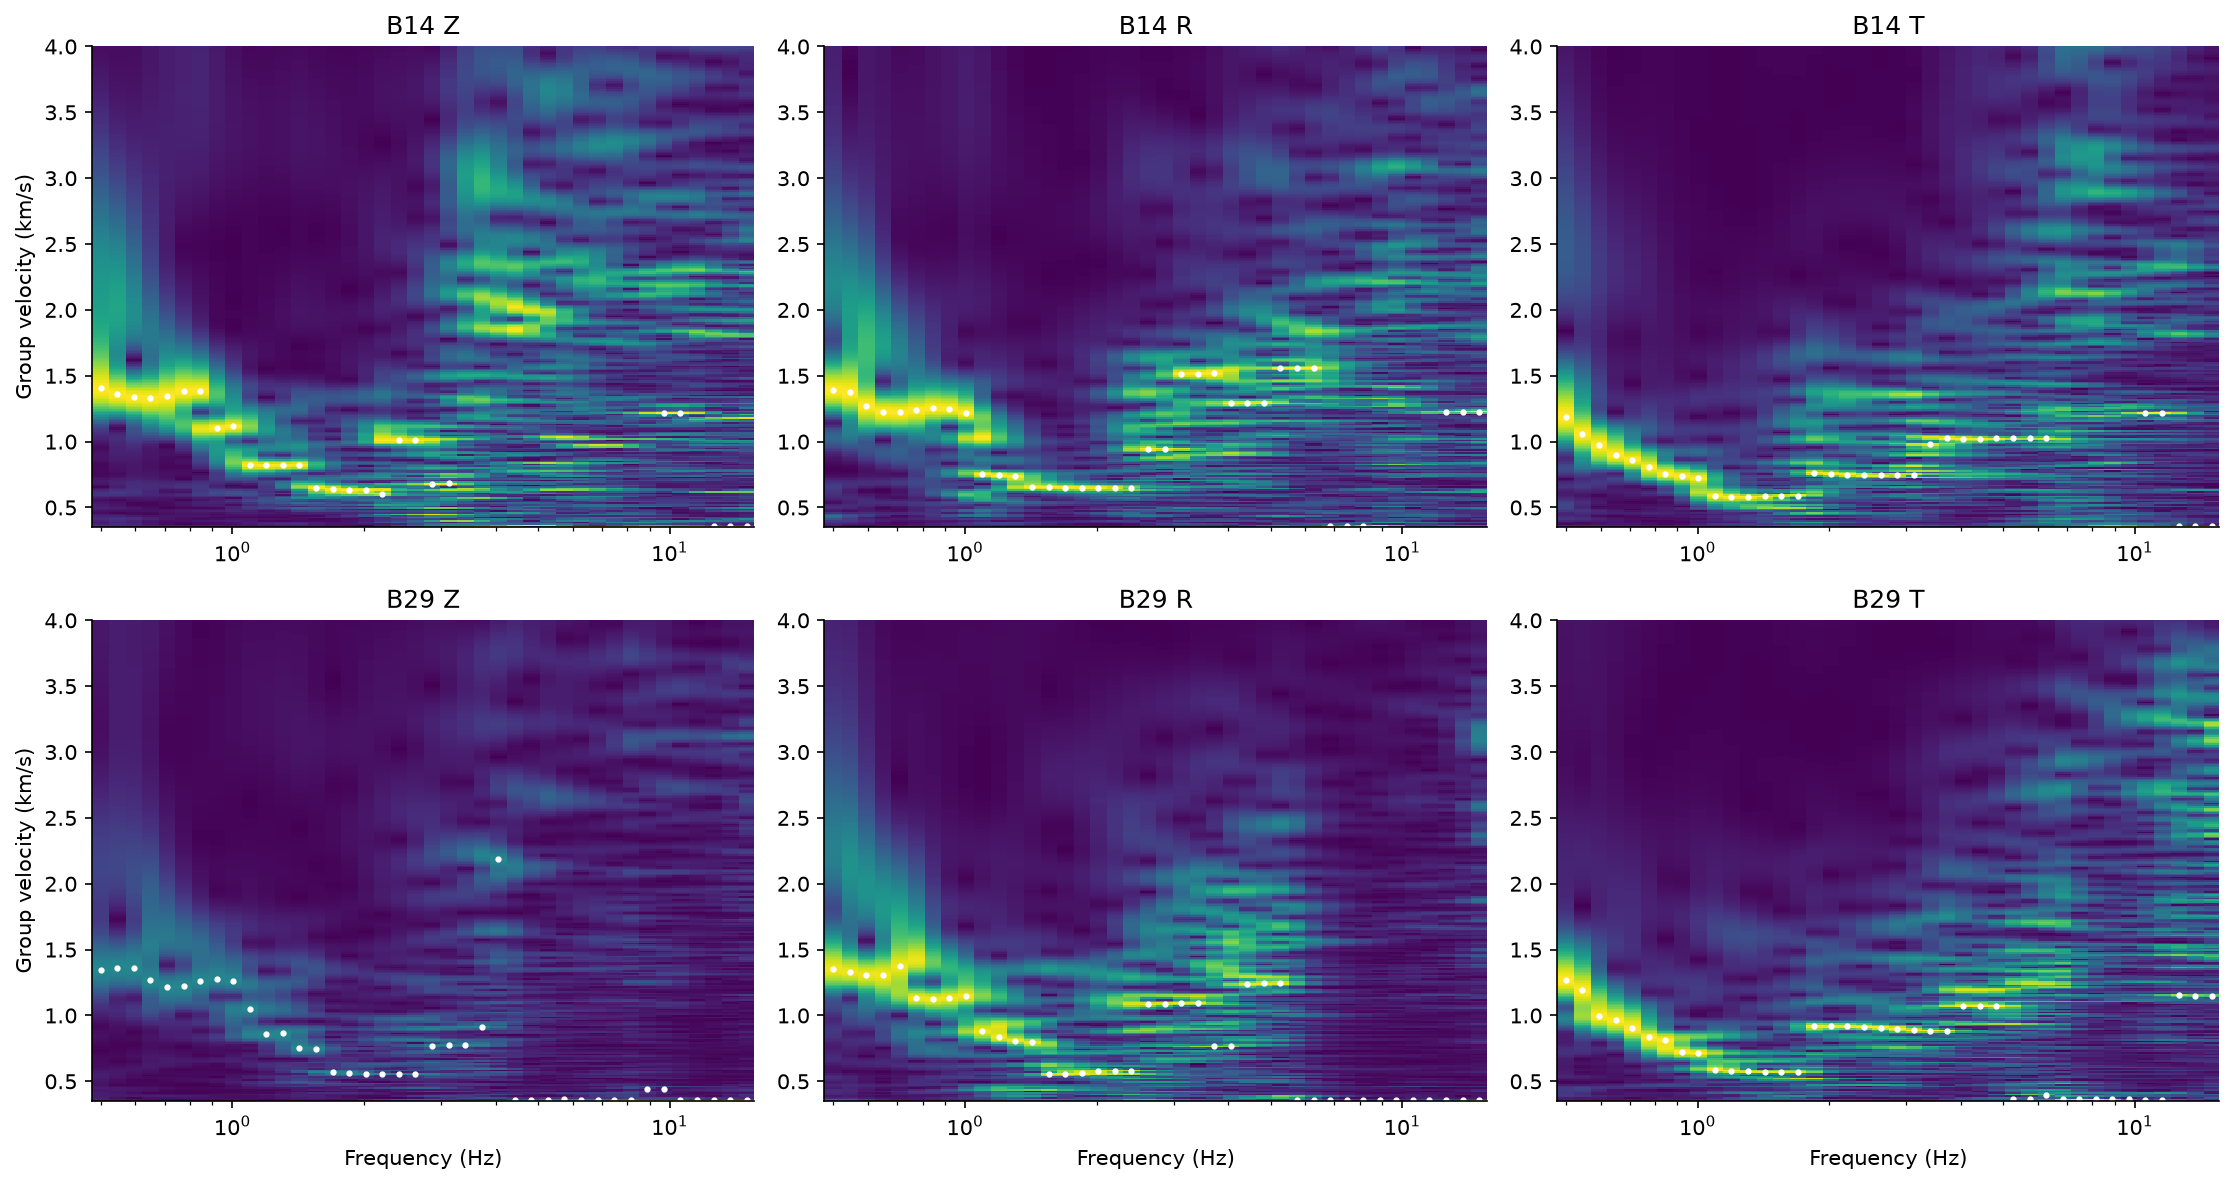
\includegraphics[width=\textwidth]{ftan_ZRT}
  \caption{Multiple-filter analysis of the vertical (Z), radial (R) and
    transverse (T) components at B14 and B29: normalised envelope against
    group velocity and frequency, with the ridge (white).}
  \label{fig:ftan}
\end{figure*}

\subsection{A first velocity model}

We fitted the Rayleigh group velocities (0.5--3.4~Hz), the fundamental
Love group velocities (0.5--1.8~Hz) and the P first arrivals with flat
models of three layers over a half-space, with $V_P = \max(1600\
\mathrm{m\,s^{-1}}, 1.9V_S)$ and densities rising from 1800 to
2250~kg~m$^{-3}$, by differential evolution. Dispersion was computed
with \texttt{disba} \citep{luu2021disba}, checked against an independent
thin-layer solver \citep{lysmer1970}. Two fits, without and with the H/V
ratio, agree on the main structure (Figure~\ref{fig:model}): a surface
layer \NGtopThick~m thick with $V_S = {}$\NGvsTop~m~s$^{-1}$, a layer of about
\NGlayerTwoThick~m at $V_S \approx{}$\NGlayerTwoVs~m~s$^{-1}$, a layer of \NGlayerThreeThick~m at
\NGlayerThreeVs~m~s$^{-1}$, and a half-space at $V_S \approx{}$
\NGvsHalf~m~s$^{-1}$ ($V_P \approx{}$\NGvpHalf~km~s$^{-1}$) from \NGhalfDepth~m depth (\supptab{13}; dispersion data in \supptab{14}).
The half-space P speed matches the first arrivals. Fitting Love and
Rayleigh waves together removes much of the trade-off of a fit to the
verticals alone, which gives a single layer of $V_S \approx{}$
\NGvertVs~km~s$^{-1}$ down to $\sim$\NGvertDepth~m (\suppfig{7}).

\begin{figure*}[htbp]
  \centering
  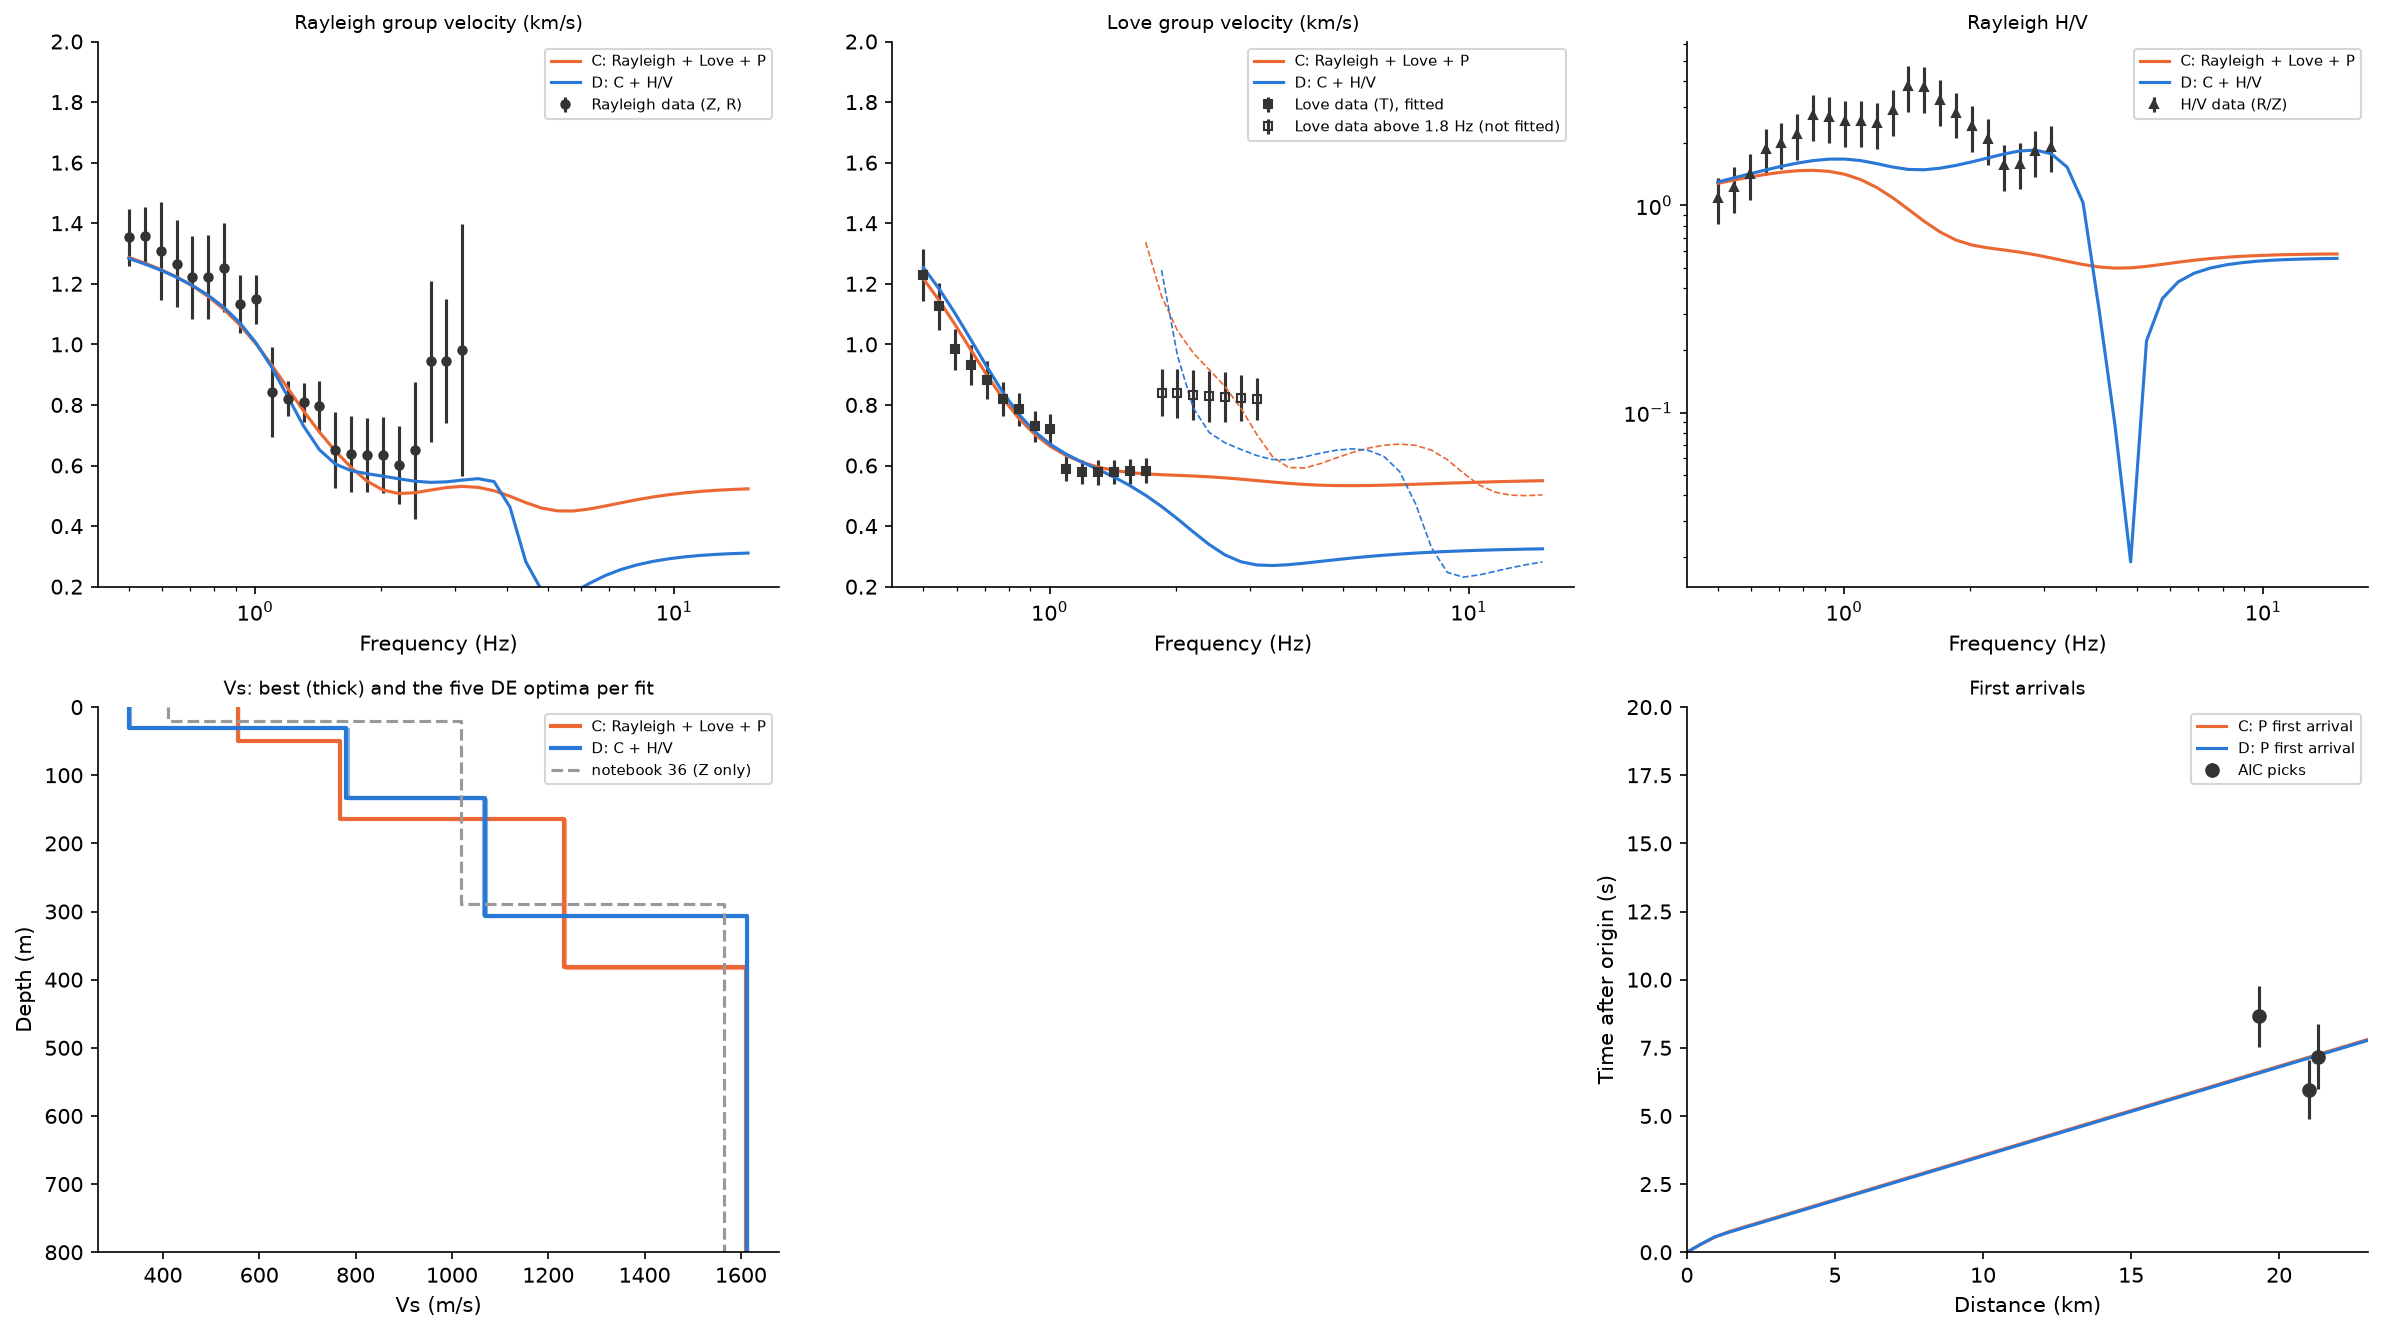
\includegraphics[width=\textwidth]{joint_model}
  \caption{Joint velocity model. Data and model predictions for Rayleigh
    group velocity, Love group velocity (open squares: above 1.8~Hz, not
    fitted; dashed: first higher mode) and Rayleigh H/V; shear-wave
    velocity profiles from fits without (orange) and with (blue) H/V, and
    from the verticals only (grey dashed); and P first arrivals.}
  \label{fig:model}
\end{figure*}

These shear-wave speeds point to lithified carbonate within a few tens
of metres of the surface and a stiffer unit near \NGhalfDepthRound~m. Assigning
them to the Hawthorn Group, the Ocala Limestone and the Avon Park
Formation needs borehole logs. From Rayleigh waves of the Artemis~I
launch recorded 2.87~km from LC-39A, \citet{woo2024geoconvention} placed
the Anastasia Formation/surficial-aquifer boundary near 9~m and the
Ocala/Hawthorn boundary near 50~m. Their group velocities
(0.09--0.16~km~s$^{-1}$ at 1--25~s) are an order of magnitude below ours,
plausibly because travel times measured from lift-off of a moving,
long-lasting source give lower bounds, whereas the explosion has an
impulsive origin. The \NGfzero~Hz ground resonance (Section~\ref{sec:coupling})
is too high for the surface layer of our models, and may reflect a
thinner, slower layer, such as that near 9~m, which waves below 3.4~Hz
cannot resolve.

%% ============================================================
\section{Discussion}

\paragraph{Yield from near-field infrasound.} Four working infraBSUs at
\NGdistRangeRound~km, with a weather-based origin time, give a yield within \NGyieldVsSilber\% of
an estimate from dozens of regional stations, using only the peak
overpressure and a standard blast relation. The positive-phase duration
gives a larger value, as expected for a propellant explosion. The main
near-field uncertainties are instrumental: relative calibration (up to
$\sim$\NGbCal\% between co-located sensors), the sampling rate (up to \NGdecMax\% on
peaks at 100~samples~s$^{-1}$) and polarity, all of which the network
can now correct.

\paragraph{Timing the source.} Near-field airwave onsets with a
weather-based sound speed time the explosion to about a second. That is
precise enough to compare with video, but only after allowing for the
supersonic blast front, which at this yield advances the arrivals by
\NGadvanceAll~s, even at 12--21~km. With that correction the airwave
comes from the main flash \citep{silber_scamfer_newglenn_2026}, not from
the fireball that preceded it by several seconds.

\paragraph{The seismic wavefield.} The explosion shows that the shallow
structure around KSC can be studied with the network's own sources when
they are impulsive and distant. A precise orientation of the
horizontals from many sources at known pads, the MSFC stations if their
data can be recovered, and launch-generated surface waves recorded
across the network would extend the single-path model presented here.
The \NGpScatter~s scatter of the P picks at \NGfarRange~km is larger than any flat
model allows and suggests lateral variation.

\paragraph{Compliance as a site property.} The air-coupled ground motion
at \NGdistRangeRound~km is a quasi-static response to the pressure load. Its
compliance agrees between a launch and an explosion at the same sites,
unlike the conventional coupling ratio, and can be compared directly
with models of the near-surface \citep{novoselov_ground_coupling_2020}.

\paragraph{Lessons for unattended networks.} Three of seven stations had
no sensors connected; three infrasound channels had reversed polarity; a
Chaparral sensor clipped and was faulty for ten weeks; and a seismometer
recorded identical horizontals all year. Each was found only because a
large, well-located signal arrived at every station. Routine checks of
noise spectra, inter-channel correlation and co-located sensor ratios
would find them earlier.

\paragraph{Limitations.} Four working stations, three of them at nearly
the same distance, constrain amplitude decay and structure only along a
narrow range of paths. The relative infraBSU calibrations, the yield
relations' extrapolation, and the 1D velocity model's assumptions (fixed
$V_P$ and density) are the main uncertainties.

%% ============================================================
\section{Conclusions}

\begin{itemize}
  \item \NGnStationsCap{} broadband stations at \NGdistRange~km recorded the New~Glenn
    static-fire explosion; \NGnWorking{} had working sensors. The airwave and
    surface weather place the origin at \NGorigin~UTC~$\pm$~1~s on
    29~May~2026, or \NGoriginCorrRange{} after allowing for the supersonic blast
    front, matching the main flash seen on video.
  \item Peak overpressures were \NGpBtwenty~Pa at \NGdistBtwenty~km and \NGpFar~Pa at
    \NGfarRange~km. Below 4~Hz the airwave decays close to spherical
    spreading; above 4~Hz it barely decays. The peak-overpressure yield,
    about \NGyieldP~t TNT, agrees with the 131~t estimated from regional
    infrasound.
  \item The airwave loads the ground quasi-statically. The compliance
    (\NGcompRange~nm~Pa$^{-1}$) is the same for a launch and an explosion at
    the same site, and is the quantity to compare between events.
  \item P waves (\NGvFirst~km~s$^{-1}$) and dispersed Rayleigh and Love
    waves arrive \NGlead~s ahead of the airwave, the first clean
    separation of the two wavefields at KSC. They give shear-wave speeds
    rising from \NGvsTop~m~s$^{-1}$ near the surface to about
    \NGvsHalfRound~m~s$^{-1}$ below \NGhalfDepth~m.
  \item The explosion exposed disconnected sensors, reversed infrasound
    polarity, a faulty Chaparral sensor and a miswired seismometer,
    problems that routine checks of an unattended network should catch.
\end{itemize}

%% ============================================================
\section*{Data and Code Availability}

Waveform data will be archived through EarthScope upon publication.
The analysis (notebooks 05--42 in \texttt{10\_NewGlenn\_paper}, built on
the shared \texttt{ksclib} package in the same repository) is available
at \url{https://github.com/gthompson/KSCRocketSeismology}; the version used will be archived with a DOI on
acceptance. Weather observations
are from the Iowa Environmental Mesonet \citep{iem_asos} and the KSC
Spaceport Weather Archive \citep{ksc_wxarchive}, and the 2026
launch list from Launch Library~2 \citep{launchlibrary2}. The analysis
builds on ObsPy \citep{Beyreuther2010,krischer_obspy_2015}, FlovoPy
\citep{flovopy_2026} and \texttt{disba} \citep{luu2021disba}.

\begin{acknowledgements}
We thank Robert G. Brown and John Kiriazes (Florida Space Institute, University of Central Florida) for
retrieving the station data within days of the explosion, and for their long experience with these stations.
We thank the Kennedy Space Center and Cape Canaveral Space Force Station personnel who made the network's
installation and servicing possible. The network was installed for the Artemis~II launch with the support of
NASA Marshall Space Flight Center; the EarthScope Primary Instrument Center and Boise State University lent the
temporary instruments for that deployment. Weather observations are from the Iowa Environmental Mesonet.
\end{acknowledgements}

\section*{Funding}

This analysis received no dedicated funding.

\bibliography{references}

\end{document}
